\documentclass[a4paper]{article}
\usepackage[utf8]{inputenc} %Input encoding

\usepackage{amsmath} %Extra math symbols and operators
\usepackage{amssymb}
\usepackage{amsthm}
\usepackage{eufrak}
\usepackage{xcolor}
\definecolor{mygray}{gray}{0.95}

\usepackage{float}

\usepackage{bm} %Bold symbols

\usepackage{graphicx} %Images

\usepackage{tikz-cd} %Diagrams

\usepackage{enumitem} %Enumerate Labels

\usepackage[margin=1.4in]{geometry} %Adjust Margins

\usepackage{siunitx} % easily format numbers with dimensions
\usepackage{hyperref}
\usepackage{cleveref}
\usepackage[textsize=tiny]{todonotes}
\usepackage{verbatim}

\usepackage[margin=20pt]{caption} %Smaller captions

\usepackage{minted} % Code highlighting

\usepackage{fancyhdr}
\pagestyle{headings}

%\usepackage{fancyhdr} %Name on every page
%\pagestyle{fancy}
%\lhead{Rune Buckinx}

\usepackage{mdframed}
\newmdtheoremenv{definition}{Definition}[section]
\newmdtheoremenv{question}{Question}[section]
\newmdtheoremenv{lemma}{Lemma}[section]
\newmdtheoremenv{proposition}{Proposition}[section]
\newtheorem{example}{Example}[section]
\newtheorem{remark}{Remark}[section]
\newmdtheoremenv{theorem}{Theorem}[section]
\newmdtheoremenv{exercise}{Exercise}

\usepackage{import}
\usepackage{xifthen}
\usepackage{pdfpages}
\usepackage{transparent}


\newcommand{\incfig}[1]{
    \def\svgwidth{\columnwidth}
    \import{./figures/}{#1.pdf_tex}
}

\usepackage[backend=biber, style = alphabetic]{biblatex}
\addbibresource{references.bib}
%\tikzset{component/.style={draw,thick,circle,fill=white,minimum size =0.75cm,inner sep=0pt}}
%\renewcommand{\thefigure}{\arabic{section}.\arabic{figure}}
\numberwithin{figure}{section}
\numberwithin{equation}{section}


\title{Modeling of MHD waves in the solar corona}
\author{Micha\"el Maex \and Rune Buckinx}
\date{March 2020}

\pagenumbering{roman}
\begin{document}

\maketitle

\begin{abstract}
    This paper presents a summary of research for a bachelor's thesis on the modelling of magnetohydrodynamic waves in the solar corona using numerical simulations via the open source code PLUTO. 
\end{abstract}
\newpage
\tableofcontents

\pagebreak

\listoffigures

\listoftodos

\newpage
\pagenumbering{arabic}
\section{Introduction} \label{sec:introduction}
The Sun's corona, or solar corona, is the outer layer of the Sun's atmosphere, which consists of fully ionized material due to it having very high temperatures compared to the surface of the sun. 
As the particles of this fluid are charged the fluid interact with the magnetic field and electric currents in the fluid have to be taken into account.  
The plasma in the solar corona can be described using magnetohydrodynamic (MHD) equations, which combine the Navier-Stokes equations from fluid dynamics with the Maxwell equations from electromagnetism. 
This approach to model the plasma treats it as a single fluid, as opposed to the two-fluid model, which describes the positive and negative charges separately. \\

The differential/governing equations that make up the MHD model, are difficult to solve analytically. 
It is therefore often favourable to use numerical computer modelling to study the equations, which is the main focus of this bachelor's project. 
The simulations will be performed in the open source code PLUTO, which is designed to solve systems of partial differential equations in astrophysical fluid dynamics \cite{mignone2011pluto}.\\

The goals of this bachelor's project are to gain familiarity with simulating and modelling phenomena, and in particular MHD waves, using numerical models and code such as PLUTO, and to gain some basic knowledge on MHD waves by analysing simulations. Concretely, this consists of the following two problems, simulating a magnetohydrodynamic blastwave and simulating the interaction of magnetohydrodynamic waves with large scale structures in the solar corona, such as a coronal hole and plume.

\pagebreak
\section{(M)HD Theory} \label{sec:(m)hd_theory}

First a brief introduction to non-magnetic hydrodynamics is given which will then be compared to magnetohydrodynamics.

\subsection{Ordinary Hydrodynamics} \label{sec:ordinary_hydrodynamics}

Fluids are described using the Navier Stokes equations. In the case of an ideal fluid these equations are referred to as the Euler equations and take the form \cite[section 1.3]{acheson1990}:

\begin{align*}
	&\text{conservation of mass:} &\frac{\partial \rho}{\partial t} + \rho \nabla \cdot \mathbf v &=  0 \\
				    &\text{conservation of momentum:} &\rho \frac{\partial \mathbf v}{\partial t} + \nabla p &= 0\\
				    &\text{conservation of enery/adiabatic equation:} &\frac{\partial }{\partial t} \left( \frac{p}{\rho^{\gamma}} \right)  &= 0
,\end{align*}
where $\mathbf v$ is the velocity,  $\rho$ is the denisity, $p$ is the pressure and $\gamma$ is the ratio of the specific heat capacities (constant pressure, constant volume) which in this report will always be $5 / 3$. 
These equations are differential forms of conservation laws. 

In a linear approximation ($p, \rho$ are small deviations of some constant background pressure and density $p_0, \rho_0$) the group speed of a wave (the speed at which a wave packet travels, energy moves) is independent of wavelength and direction. It is usually referred to as the speed of sound and is given by\cite[section 3.6]{acheson1990} \[
c_s = \sqrt{\gamma \frac{p_0}{\rho_0}} 
.\] 

\subsection{Magnetohydrodynamics and the solar corona} \label{sec:magnetohydrodynamics_and_the_solar_corona}
The classic Navier-Stokes equations do not suffice to describe the movement in the solar corona due to the influence of strong magnetic fields on the ionized particles. This magnetic field stems from convection in the photosphere, which is a physical process that helps transport the nuclear energy created in the core of the sun \cite{brun2017magnetism}.\\

The use of the magnetohydrodynamic model to describe the plasma depends on three main assumptions, namely, high collisionality, large scales and the assumption of ideal fluids. The last assumption implies that the dissipation of large scale variables is neglected \cite{goedbloed2004principles}. This model also does not take relativity into account, as opposed to the relativistic magnetohydrodynamic model, which will not be discussed further\footnote{More information about the relativistic MHD model can be found in \cite{karas2005introduction}}. The non-relativistic approximation is valid when the speeds considered are much smaller than the speed of light, which will be the case throughout this report.

\todo{Afleiding vanuit conservatiewetten nodig? Enkel als we echt paginas te kort komen}
The system of PDE's/conservations laws is the following:
\begin{alignat}{3}
    &\frac{\partial \rho}{\partial t} &&+ \rho \nabla  \cdot (\mathbf v) &&= 0 \tag{mass}\label{eq:mass}\\
    \rho&\frac{\partial \mathbf v}{\partial t} &&+  \nabla p - \frac{(\nabla \times \mathbf{B}) \times \mathbf{B}}{\mu} &&= 0 \tag{moment}\label{eq:cauchymoment}\\
    &-\frac{\partial \mathbf B}{\partial t} &&+ \nabla \times (\mathbf{v} \times \mathbf{B}) &&= 0 \tag{charge}\label{eq:faraday}\\
    &\frac{\partial}{\partial t}\left(\frac{p}{\rho^\gamma}\right) && &&= 0 \tag{energy}\label{eq:energy}.
\end{alignat} 
Here $\rho$ is the plasma density, $\mathbf B$ is the magnetic field,  $\mathbf v$ the velocity, $p$ is the thermal pressure. The constant $\mu$ is the magnetic permeability. 

There are similarities to Euler equations (\cref{sec:ordinary_hydrodynamics}).
The third equation models the interaction between the currents in the plasma and the magnetic field and orginates in the Maxwell equations.
As magnetic fields can carry momentum \cite[section 8.2]{GriffithsDavidJeffery2017Ite} a term has to be added to the momentum equation. 
This term incorporates the effect of magnetic pressure the size of which is given by $P_B = \frac{B^2}{2\mu}$. 
A very important quantity often used in plasma physics is the plasma-$\beta$ which gives the ratio between ordinary/thermal pressure and magnetic pressure. It is defined as \[
\beta = \frac{p}{P_B} = \frac{2 \mu p}{B^2}
.\] 
If $\beta \gg 1$ the pressure dominates and the magnetic effects can be ignored. If $\beta \ll 1$ the magnetic pressure dominates.
\subsection{Linear Approximations} \label{sec:linear_approximations}

To analyse small amplitude waves in the plasma, a linearised version of the magnetohydrodynamic equations is considered as in \cite{Fitzpatricknotes}, namely

\begin{alignat}{3}
    &\frac{\partial \rho_1}{\partial t} &&+ \rho_0 \nabla  \cdot (\mathbf v_1) &&= 0 \tag{mass}\label{eq:masslin}\\
    \rho_0&\frac{\partial \mathbf v_1}{\partial t} &&+  \nabla p_1 - \frac{(\nabla \times \mathbf{B_1}) \times \mathbf{B_0}}{\mu} &&= 0 \tag{moment}\label{eq:cauchymomentlin}\\
    &-\frac{\partial \mathbf B_1}{\partial t} &&+ \nabla \times (\mathbf{v_1} \times \mathbf{B_0}) &&= 0 \tag{charge}\label{eq:faradaylin}\\
    &\frac{\partial}{\partial t}(\frac{p_1}{p_0} - \frac{\gamma\rho_1}{\rho_0}) && &&= 0 \tag{energy}\label{eq:energylin}.
\end{alignat}

Where $\mu$ is the vacuum permeability constant, and initial flow velocity and plasma current are assumed to be zero. This linearisation is done by writing the physical quantities as
\begin{equation*}
    f(\mathbf{x},t) = f_0(\mathbf{x}) + f_1(\mathbf{x},t)
\end{equation*}
under the assumption that the perturbation ($f_1$) of the equilibrium ($f_0$) is small compared to this equilibrium.
The further analysis is based on the online lecture notes by R. Fitzpatrick \cite{Fitzpatricknotes}.\\

Consider perturbations of the following form, $\exp(i(\mathbf{kx} + \omega t))$, substituting this in the equations results in the following system of equations,

\begin{alignat}{3}
    &-\omega\rho_1 &&+  \rho_0 \mathbf{k}\cdot\mathbf v_1 &&= 0 \label{eq:MHD_linear_wave_mass}\\
    &-\omega\rho_0\mathbf v_1 &&+  \mathbf{k} p_1 - \frac{(\mathbf{k} \times \mathbf{B_1}) \times \mathbf{B_0}}{\mu} &&= 0 \label{eq:MHD_linear_wave_moment}\\
    &-\omega\mathbf B_1&&+ \mathbf{k} \times (\mathbf{v_1} \times \mathbf{B_0}) &&= 0 \label{eq:MHD_linear_wave_charge}\\
    &-\omega(\frac{p_1}{p_0} - \frac{\gamma\rho_1}{\rho_0}) && &&= 0  \label{eq:MHD_linear_wave_enery}.
\end{alignat}

Rewriting these equations in function of the equilibrium states and $\mathbf{v_1}, \mathbf{k}$ and $\omega$ leads to,
\begin{align*}
    \rho_1 &= \rho_0 \frac{\mathbf{k} \cdot \mathbf{v_1}}{\omega}\\
    p_1 &= \gamma p_0 \frac{\mathbf{k} \cdot \mathbf{v_1}}{\omega}\\
    \mathbf{B_1} &= \frac{(\mathbf{k} \cdot \mathbf{v_1}) \cdot \mathbf{B_0} - (\mathbf{k} \cdot \mathbf{B_0})\cdot \mathbf{v_1}}{\omega}
\end{align*}
These values can now be subsituted in the linearised moment equation yielding the following,
\begin{equation*}
    -\omega\rho_0\mathbf{v_1} + \mathbf{k}\cdot \frac{\gamma p_0}{\omega}-\frac{(k\times \frac{(\mathbf{k} \cdot \mathbf{v_1}) \cdot \mathbf{B_0} - (\mathbf{k} \cdot \mathbf{B_0})\cdot \mathbf{v_1}}{\omega})\times \mathbf{B_0}}{\mu} = 0
\end{equation*}
Further rearranging of the terms gives,
\begin{equation} \label{eq:linearised_mhd_5}
	\bigg(\omega^2 - \frac{(\mathbf{k \cdot B_0)^2}}{\mu\rho_0}\bigg)\mathbf{v_1} 
	= \bigg[\bigg(\frac{\gamma p_0}{\rho_0}- \frac{\mathbf{B_0}^2}{\mu\rho_0}\bigg)\mathbf{k} + \frac{(\mathbf{k \cdot B_0)}}{\mu\rho_0}\mathbf{B_0}\bigg](\mathbf{k\cdot v_1}) 
	- \frac{(\mathbf{k \cdot B_0})(\mathbf {v_1}\cdot \mathbf{B_0})}{\mu\rho_0}\mathbf{k}
\end{equation}
To simplify further notation, $c_s = \sqrt{\frac{\gamma p_0}{\rho_0}}$ will be used to represent the sound speed, and $v_A = \sqrt{\frac{\mathbf{B_0}^2}{\mu\rho_0}}$ will be used to represent the ``Alfv\'en speed''. Let $\theta$ be the angle between $\mathbf{B_0}$ and $\mathbf k$. \Cref{eq:linearised_mhd_5} then becomes
\begin{equation}
	\left( \omega^2 - v_A^2 \cos^2\theta \right)k^2 \mathbf{v_1}  
	- \left[ (c_s^2 + v_A^2) \mathbf k - v_A^2\cos\theta \frac{k}{B_0}\mathbf{B_0} \right](\mathbf k \cdot \mathbf{v_1}) 
	+ v_A^2\cos\theta \frac{k}{B_0}(\mathbf{v_1}\cdot \mathbf{B_0}) \mathbf k
	=0
\end{equation}
Under the assumption that the magnetic field lies in the $x$-direction, and the wave front vector $k$ lies in the $x,y$-plane this can be rewritten as follows, where $\theta$ represents the angle between $\mathbf{B_0}$ and $\mathbf{k}$, i.e. $k_x = k\cos\theta , k_y = k \sin\theta, k_z = 0$.
\begin{align*}
	&\left( \omega^2 - k^2v_A^2\cos^2\theta \right) \mathbf I_3 \begin{pmatrix} v_x \\ v_y \\ v_z \end{pmatrix} \\
	- &k^2\left[ (c_s^2 + v_A^2) \begin{pmatrix} \cos \theta \\ \sin\theta \\ 0 \end{pmatrix} - v_A^2\cos\theta  \begin{pmatrix} 1 \\ 0 \\ 0 \end{pmatrix}  \right] \begin{pmatrix} \cos \theta & \sin \theta & 0 \end{pmatrix} \begin{pmatrix} v_x \\ v_y \\ v_z \end{pmatrix} \\
	+ &k^2v_A^2 \cos\theta \begin{pmatrix} \cos\theta \\ \sin \theta \\ 0  \end{pmatrix} \begin{pmatrix} 1 & 0 & 0 \end{pmatrix} \begin{pmatrix} v_x \\ v_y \\ v_z  \end{pmatrix}  \\
	&=  \mathbf 0
\end{align*}

Writing every term as a matrix yieldsc:
\begin{align*}
	&\begin{pmatrix}
		\omega^2  - k^2 v_A^2 \cos\theta^2    & 0 & 0 \\
		0 & \omega^2 - k^2v_A^2\cos^2\theta & 0 \\
		0 & 0 & \omega^2 - k^2v_A^2\cos^2\theta
	\end{pmatrix} 
	\begin{pmatrix} v_x \\ v_y \\ v_z \end{pmatrix} \\
	 & + \begin{pmatrix} 
		 -k^2 c_s^2 \cos^2 \theta & - k^2 c_s^2 \cos\theta \sin \theta  & 0 \\
		 -k^2(c_s^2 + v_A^2) \cos\theta \sin \theta & -k^2(c_s^2 + v_a^2) \sin^2\theta & 0 \\
		 0 & 0 & 0
	 \end{pmatrix} \begin{pmatrix} v_x \\ v_y \\ v_z \end{pmatrix} \\  
	 &  + \begin{pmatrix} 
		 k^2 v_a^2 \cos^2\theta & 0 & 0  \\
		 k^2 v_a^2 \cos \theta \sin \theta & 0 & 0 \\
		 0 & 0 & 0
	 \end{pmatrix} \begin{pmatrix} v_x \\ v_y \\ v_z \end{pmatrix} 
\end{align*}
This yields:
\begin{equation}\label{eq:MHD_linear_matrix}
	\begin{pmatrix}
		\omega^2  - k^2 c_s^2 \cos^2\theta   & -k^2c_s^2\cos\theta \sin \theta & 0 \\
		-k^2 c_s^2 \cos\theta \sin \theta & \omega^2 - k^2(c_s^2\sin^2\theta - v_A)   & 0 \\
		0 & 0 & \omega^2 - k^2v_A^2\cos^2\theta
	\end{pmatrix} 
	\begin{pmatrix} v_x \\ v_y \\ v_z \end{pmatrix} 
	 = \begin{pmatrix} 0 \\ 0 \\0  \end{pmatrix} 
\end{equation}
For this to be satisfied, the determinant of the matrix on the left hand side must be zero. 
\[
	(\omega^2 - k^2v_A^2 \cos \theta)\left[ (\omega^2-k^2c_s^2 \cos^2 \theta)(\omega - k^2c_s^2 \sin^2 \theta + k^2 v_A) - k^4c_s^{4}\cos^2\theta \sin^2\theta   \right] = 0
.\] 
Simplifying this results in the dispersion relation for plasma waves
\begin{equation}\label{eq:disperion}
	(\omega^2 - k^2 v_A^2 \cos^2 \theta)\left[ \omega^{4} - \omega^2k^2(v_A^2 + c_s^2) + k^{4}v_A^2c_s^2\cos^2\theta \right]  = 0
.\end{equation} 
This relation has three roots for $\omega^2$ that correspond to three different kinds of waves:\todo{refactor acoustic to magneto-sonic}
\begin{align*}
	\omega^2 &=  k^2v_a^2\cos^2\theta \tag{Alfv\'en Waves} \\
	\omega^2 &= \frac{k^2}{2}\left( v_A^2 + c_s^2 + \sqrt{(v_A^2 + c_s^2)^2 - 4v_A^2c_s^2\cos^2\theta}  \right) \tag{Fast magnetosonic waves}\\
	\omega^2 &= \frac{k^2}{2}\left( v_A^2 + c_s^2 - \sqrt{(v_A^2 + c_s^2)^2 - 4v_A^2c_s^2\cos^2\theta}  \right) \tag{Slow magnetosonic waves}
.\end{align*}
\subsection{Alfv\'en Waves}
The previous derivation led to two different types of waves, namely, Alfv\'en waves and sound waves. An Alfv\'en wave is a magnetic tension wave caused by a restoring force. 
This force follows from Lenz's law, which states that the electrical currents caused by the motion of a conducting fluid in a magnetic field give rise to a force countering this motion, and Newton's second law for fluids \cite{Finlay2007}. 
Properties of Alfv\'en waves are that they travel along the magnetic field lines and hence cannot propagate across field lines and that they do not perturb density \cite{mhdppt}.\\


Alfv\'en waves occur when \[
\omega^2 = k^2v_a^2\cos^2 \theta
.\] 
As can be seen from \cref{eq:MHD_linear_matrix} the corresponding eigenvector is in the $z$-direction \[
	\mathbf{v_1} = v \begin{pmatrix} 0 \\ 0 \\ 1 \end{pmatrix} 
.\] 
As a result $\mathbf k \cdot \mathbf{v_1} = 0$ and \cref{eq:MHD_linear_wave_mass} implies that the perturbation in density, $\rho_1  = 0$. \Cref{eq:MHD_linear_wave_enery} states that $p_1$ vanishes as well. 
As $\mathbf{B_0}$  and $\mathbf{V_1}$ lie in the $x$ and $z$-direction respectively, $\cref{eq:cauchymomentlin}$ and $\cref{eq:faradaylin}$ simplify to
\begin{align*}
	\rho_0 \frac{\partial v_z}{\partial t} - \frac{B_1}{\mu} \frac{\partial B_0}{\partial x} &= 0 \\
	\frac{\partial B_x}{\partial t}  + B_0\frac{\partial v_z}{\partial t} 
.\end{align*}
The phase velocity of an Alfv\'en wave is equal to $\omega/k$ or,
\begin{equation*}
    v_{\text{ph}} = \omega/k = v_A \cos\theta.
\end{equation*}
The group velocity is equal to a constant, namely the Alfv\'en speed.
\begin{equation*}
    v_{\text{gr}} = v_A
\end{equation*}
The comparison of this kind of wave with the fast and slow acoustic waves is made in the Friedrich diagrams below.
\subsection{Magnetosonic Waves}
The second type of wave found in the dispersion relation are magnetosonic waves. There are two roots corresponding to this type of wave of which one is faster than the other, they correspond to what is called the fast magnetosonic wave and the slow magnetosonic wave.\\

The eigenvector linked to the magnetosonic waves is in the $x,y$-plane, as can be seen from \cref{eq:MHD_linear_matrix}.
\[
	\mathbf{v_2} = v \begin{pmatrix} 1 \\ 1 \\ 0 \end{pmatrix} 
.\] 
In this case $\mathbf{k\cdot v_2}$ and $\mathbf{v_2 \cdot B_0}$ do not vanish implying that the waves cause perturbations in the density and the pressure of the plasma.

The phase velocity can again be calculated by dividing $\omega$ by $k$, this results in,
\begin{equation}\label{eq:phase_velocity}
\begin{split}
    v_{\text{phF}} &= \omega/k = \sqrt{\frac{1}{2}\left(v_A^2 + c_s^2 + \sqrt{(v_A^2 + c_s^2)^2 - 4v_A^2c_s^2\cos^2\theta}\right)}\\
    v_{\text{phS}} &= \omega/k = \sqrt{\frac{1}{2}\left(v_A^2 + c_s^2 - \sqrt{(v_A^2 + c_s^2)^2 - 4v_A^2c_s^2\cos^2\theta}\right)}
\end{split}
\end{equation}
\Cref{fig:friedrich_diagrams} shows the phase speed of the slow, fast and Alfv\'en waves for different ratios of $v_A / c_s$. 
\begin{figure}[h]
	\centering
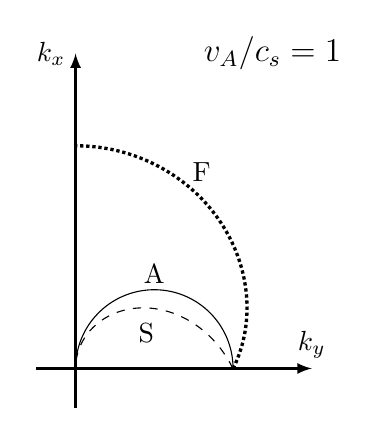
\begin{tikzpicture}
  \draw[thick,->,>=latex] (-0.5,0)--(3,0) node[above] {$k_y$};
  \draw[thick,->,>=latex] (0,-0.5)--(0,4) node[left] {$k_x$};
  \draw[domain=0:1/2*pi,scale=2,samples=500] plot (xy polar cs:angle=\x r, radius={cos(\x r)});
  \draw[domain=0:1/2*pi,scale=2,samples=500, densely dotted, very thick] plot (xy polar cs:angle=\x r, radius={sqrt((1/2)*(2+sqrt(4-4*cos(\x r)^2)))});
  \draw[domain=0:1/2*pi,scale=2,samples=500, dashed] plot (xy polar cs:angle=\x r, radius={sqrt((1/2)*(2-sqrt(4-4*cos(\x r)^2)))});
  \node at (1,1.2) {A};
  \node at (0.9, 0.45) {S};
  \node at (1.6, 2.5) {F};
  \node at (2.5,4) {\large $v_A/c_s = 1$};
\end{tikzpicture}
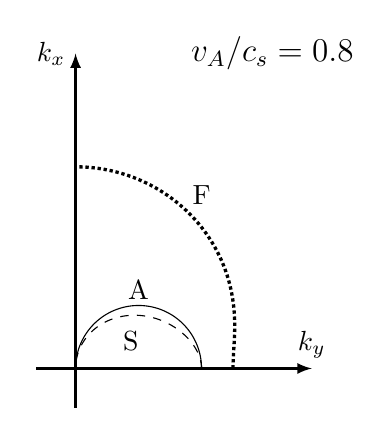
\begin{tikzpicture}
  \draw[thick,->,>=latex] (-0.5,0)--(3,0) node[above] {$k_y$};
  \draw[thick,->,>=latex] (0,-0.5)--(0,4) node[left] {$k_x$};
  \draw[domain=0:1/2*pi,scale=2,samples=500] plot (xy polar cs:angle=\x r, radius={0.8*cos(\x r)});
  \draw[domain=0:1/2*pi,scale=2,samples=500, densely dotted, very thick] plot (xy polar cs:angle=\x r, radius={sqrt((1/2)*((1.64)+sqrt((2.6896)-4*0.64*cos(\x r)^2)))});
  \draw[domain=0:1/2*pi,scale=2,samples=500, dashed] plot (xy polar cs:angle=\x r, radius={sqrt((1/2)*((1.64)-sqrt((2.6896)-4*0.64*cos(\x r)^2)))});
  \node at (0.8,1) {A};
  \node at (0.7, 0.35) {S};
  \node at (1.6, 2.2) {F};
  \node at (2.5,4) {\large $v_A/c_s = 0.8$};
\end{tikzpicture}
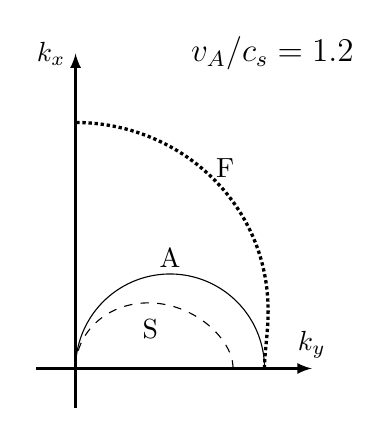
\begin{tikzpicture}
  \draw[thick,->,>=latex] (-0.5,0)--(3,0) node[above] {$k_y$};
  \draw[thick,->,>=latex] (0,-0.5)--(0,4) node[left] {$k_x$};
  \draw[domain=0:1/2*pi,scale=2,samples=500] plot (xy polar cs:angle=\x r, radius={1.2*cos(\x r)});
  \draw[domain=0:1/2*pi,scale=2,samples=500, densely dotted, very thick] plot (xy polar cs:angle=\x r, radius={sqrt((1/2)*((2.44)+sqrt((5.9536)-4*1.44*cos(\x r)^2)))});
  \draw[domain=0:1/2*pi,scale=2,samples=500, dashed] plot (xy polar cs:angle=\x r, radius={sqrt((1/2)*((2.44)-sqrt((5.9536)-4*1.44*cos(\x r)^2)))});
  \node at (1.2,1.4) {A};
  \node at (0.95, 0.5) {S};
  \node at (1.9, 2.55) {F};
  \node at (2.5,4) {\large $v_A/c_s = 1.2$};
\end{tikzpicture}
	\caption{The following diagrams represent the phase speed of the different types of magnetohydrodynamic waves plotted as radial distance. The angle between $k$ and $B_0$ is the angle away from the $k_y$ axis.}\label{fig:friedrich_diagrams}
\end{figure}

The derivation for the group velocity takes more steps, and is based on the derivation in \cite{Lyu2014}. For any wave it is defined as 
\begin{equation*}
    v_{\text{gr}} = \frac{d\omega}{d\mathbf{k}} = \hat{k}\frac{\partial\omega}{\partial k} + \hat{\theta} \frac{1}{k}\frac{\partial\omega}{\partial\theta}
\end{equation*}
The $k$-component can be calculated as follows,
\begin{align*}
    \frac{\partial \omega}{\partial k} &= \frac{\partial}{\partial k}\left(kv_{\text{ph}}\right)\\
    &= v_{\text{ph}}
\end{align*}
Which is a function of $\theta$.\\
The $\theta$-component can be calculated by rewriting the term,
\begin{align*}
    \frac{1}{k}\frac{\partial \omega}{\partial \theta} &= \frac{\partial}{\partial \theta}\left(\frac{\omega}{k}\right)
    = \frac{\partial}{\partial \theta}(v_{\text{ph}}) = \frac{1}{2v_{\text{ph}}} \frac{\partial}{\partial \theta}(v^2_{\text{ph}})
\end{align*}
The remainder of the calculations will be done for the fast wave, the slow wave case is analogous. The partial derivative of the phase speed of the fast wave squared becomes,
\begin{align*}
     \frac{\partial}{\partial \theta}(v^2_{\text{phF}})&= \frac{1}{2}\frac{\partial}{\partial \theta} \sqrt{(v_A^2 + c_s^2)^2 - 4v_A^2c_s^2\cos^2\theta}\\
     &= \frac{2v_A^2c_s^2\cos\theta\sin\theta}{\sqrt{(v_A^2 + c_s^2)^2 - 4v_A^2c_s^2\cos^2\theta}}
\end{align*}
Substituting this back in to the equation gives,
\begin{align*}
     \frac{1}{k}\frac{\partial \omega}{\partial \theta} &= \frac{1}{v_{\text{phF}}}  \frac{v_A^2c_s^2\cos\theta\sin\theta}{\sqrt{(v_A^2 + c_s^2)^2 - 4v_A^2c_s^2\cos^2\theta}}\\
     &= \frac{1}{\sqrt{\frac{1}{2}\left(v_A^2 + c_s^2 + \sqrt{(v_A^2 + c_s^2)^2 - 4v_A^2c_s^2\cos^2\theta}\right)}}\frac{v_A^2c_s^2\cos\theta\sin\theta}{\sqrt{(v_A^2 + c_s^2)^2 - 4v_A^2c_s^2\cos^2\theta}}
\end{align*}
Combining this with the $k$-component gives the group velocity,
\begin{align*}
    v_\text{grF} = &\hat{k}\sqrt{\frac{1}{2}\left(v_A^2 + c_s^2 + \sqrt{(v_A^2 + c_s^2)^2 - 4v_A^2c_s^2\cos^2\theta}\right)}\\ &+ \hat{\theta}\frac{1}{\sqrt{\frac{1}{2}\left(v_A^2 + c_s^2 + \sqrt{(v_A^2 + c_s^2)^2 - 4v_A^2c_s^2\cos^2\theta}\right)}}\frac{v_A^2c_s^2\cos\theta\sin\theta}{\sqrt{(v_A^2 + c_s^2)^2 - 4v_A^2c_s^2\cos^2\theta}}\\
    v_\text{grS} = &\hat{k}\sqrt{\frac{1}{2}\left(v_A^2 + c_s^2 - \sqrt{(v_A^2 + c_s^2)^2 - 4v_A^2c_s^2\cos^2\theta}\right)}\\ &- \hat{\theta}\frac{1}{\sqrt{\frac{1}{2}\left(v_A^2 + c_s^2 - \sqrt{(v_A^2 + c_s^2)^2 - 4v_A^2c_s^2\cos^2\theta}\right)}}\frac{v_A^2c_s^2\cos\theta\sin\theta}{\sqrt{(v_A^2 + c_s^2)^2 - 4v_A^2c_s^2\cos^2\theta}}
\end{align*}
This can be simplified with \cref{eq:phase_velocity}:
\begin{align*}
	v_{\text{grF}} &= v_\text{phF}  \hat{k} + \frac{v_A^2c_s^2 \cos \theta \sin \theta}{v_\text{phF} \sqrt{(v_A^2 + c_s^2)^2 - 4v_A^2c_s^2 \cos^2 \theta}} \hat{\theta}\\
	v_{\text{grS}} &= v_\text{phS}  \hat{k} - \frac{v_A^2c_s^2 \cos \theta \sin \theta}{v_\text{phS} \sqrt{(v_A^2 + c_s^2)^2 - 4v_A^2c_s^2 \cos^2 \theta}} \hat{\theta}\\
\end{align*}
\Cref{fig:groupspeed_beta} shows the group speed of the slow, fast and Alfv\'en waves for different values of the plasma-$\beta$

\begin{figure}[h]
	\centering
	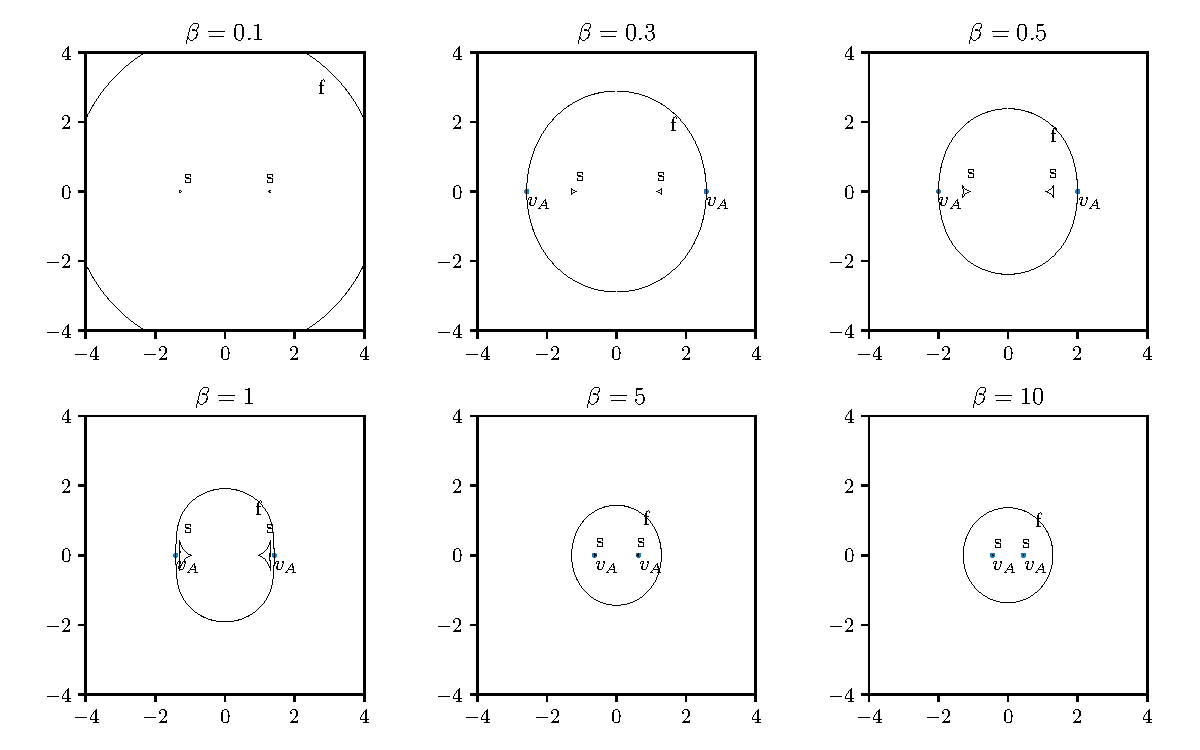
\includegraphics[width =\textwidth]{figures/groupspeed_beta.pdf}
	\caption{The possible group speeds for fast, slow and Alfv\'n waves for different values of $\beta$. The magnetic field lines are horizontal.}
	\label{fig:groupspeed_beta}
\end{figure}

\pagebreak

\section{Pluto Code} \label{sec:pluto_code}

The Pluto library consists completely out of uncompiled code. For each problem/simulation a binary needs to be made specific to that problem. This allows Pluto to be run on a large variety of devices, provided that the necessary compilers are available.
The files specific to a problem are referred to as the definition of the problem. 
This definition typically consists of three files, \texttt{definitions.h}, \texttt{init.c}, \texttt{pluto.ini}.
\begin{enumerate}
	\item \texttt{definitions.h} contains all the information necessary for compiling the right code for the project. This mostly constist of information for the solver: what solver is used (HD, MHD, relativistic MHD), what kind of grid geometry is used (number of dimensions, cartesian, cylidrical, polar), what code units represent (see \cref{sec:units_in_pluto}). It also contains what user definable variables there are.
	\item \texttt{init.c} contains the C-functions that specify initial and boundary conditions. The function \texttt{void Init (double *v, double x1, double x2, double x3)} sets up stores the initial conditions at the point \texttt{(x1,x2,x3)} and stores them in at the pointer \texttt{*v}.
		The function \texttt{void UserDefBoundary (const Data *d, RBox *box, int side, Grid *grid)} can be used to define custom boundary conditions when the build in boundary conditions (periodic, passthrough, mirror, \ldots) are not sufficient.
	\item \texttt{pluto.ini} contains information that the binary reads before starting the computation. This constists of grid size and resolution, simulation time, what output needs to be stored where and the values of the user defined parameters.
\end{enumerate}
The compiler uses \texttt{definitions.h} to only compile the right solver and \texttt{init.c}. One binary can use multiple \texttt{pluto.ini}'s which makes it easy to run multiple simulations of the same setup with different input variables. 

\subsection{Units in Pluto} \label{sec:units_in_pluto}

Internally Pluto uses dimensionless code units. All units are derived from the constants \texttt{UNIT\_DENSITY} ($\rho_0$), \texttt{UNIT\_LENGTH} ($L_0$), \texttt{UNIT\_VELOCITY} ($v_0$), all of which are denoted in cgs units. All other units are derived from these units.  
Note that the unit for magnetic field is defined as $B_0 = v_0\sqrt{4\pi \rho_0} $.

\Cref{tab:default_units} shows some important dimensions in (M)HD and what one code unit represents when \texttt{UNIT\_DENSITY}, \texttt{UNIT\_LENGTH} and  \texttt{UNIT\_VELOCITY} have their default values.
\begin{table}[htpb]
	\centering
	\caption{Important dimensions and their code units in PLUTO}
	\label{tab:default_units}
	\begin{tabular}{c|c}
		one code unit of & corresponds to\\
		\hline 
		density & $m_p$ \si{\per \centi\metre\cubed} = \SI{1.67262171e-24}{\gram \per \centi\metre\cubed}\\
		lenth &\SI{1}{AU} \\
		velocity & \SI{1}{\kilo\metre \per \second}\\
		time & \SI{149597892}{\second} \\
		magnetic field strength & \SI{4.584624773e-07}{Gs} \\
		pressure & \SI{1.67262171e-14}{Ba} = \SI{1.6726217e-15}{Pa}
	\end{tabular}
\end{table}

\subsection{Initial example} \label{sec:initial_example}
The first problem that will be analysed is a simple hydrodynamic blastwave generated by a high-pressure region. 
The viscosity, heat conduction and dissipation of the fluid will be neglected. 
This problem is meant to be an initial example of how to set up a non-predefined simulation and is a modified version of the initial example described in section 0.4 of PLUTO's User Guide \cite{plutouserguide}. 
The blastwave is simulated in two dimensions and uses three user-defined parameters, namely, the ambient pressure, the pressure in the high-pressure region, and $\gamma$ which in this report will always be $5/3$. 
The domain is a rectangle going from -10 to 10 (code units), in both the $x$ and the $y$ direction, which is represented by a $1024\times 1024$ grid. 

The following initial condition is used, a high-pressure region inside a circle of radius 0.3 is surrounded by an ambient pressure region. The simulation is run for X units of time, and every Y units, a double-precision file is saved.\\

The file \texttt{pluto.ini} stores paramters for the simulation, including grid size, grid resolution, simulation time, output format and user defined parameters. In this case can be set up in PLUTO by making the following adjustments to the \texttt{pluto.ini} file.
\begin{minted}
[frame=lines, bgcolor=mygray]
{c}
[Grid]

X1-grid    1    -10.0    1024    u    10.0
X2-grid    1    -10.0    1024    u    10.0

[Static grid output]

dbl        0.01  -1   multiple_files

[Parameters]

P_IN                        15.0  
P_OUT                       8.0  
GAMMA                       1.66666666666666667  
\end{minted}

The file \texttt{init.c} contains the code to generate the initial and boundary conditions. 
To define the problem the following adjustments have to be made to the \texttt{void init(\ldots)} function, which generates the initial conditions for a given point on the grid. 
\begin{minted}
[frame=lines, bgcolor=mygray]
{c}
void Init (double *v, double x1, double x2, double x3)
{
  double r;
  g_gamma = g_inputParam[GAMMA];
  r = x1*x1 + x2*x2;
  r = sqrt(r);

  v[RHO] = 1.0;
  v[VX1] = 0.0;
  v[VX2] = 0.0;
  v[VX3] = 0.0;
  #if HAVE_ENERGY
  v[PRS] = g_inputParam[P_OUT];
  #endif
  if (r <= 0.3) v[PRS] = g_inputParam[P_IN];
  v[TRC] = 0.0;
}
\end{minted}
\vspace{1cm}

PLUTO's hydrodynamics module solves the following system of equations

\begin{alignat}{3}
    &\frac{\partial \rho}{\partial t} &&+ \nabla \cdot (\rho \mathbf v) &&= 0 \tag{mass}\label{masscont}\\
    &\frac{\partial \mathbf m}{\partial t} &&+  \nabla \cdot (\mathbf{mv + I}p)^T &&= -\rho \nabla \Phi \tag{moment}\label{cauchymoment}\\
    &\frac{\partial(E_t + \rho \Phi)}{\partial t} &&+ \nabla \cdot ((E_t + p +\rho\mathbf{\Phi})\mathbf{v}) &&= 0 \tag{energy}\label{energy}.
\end{alignat}

These can be derived from the standard Euler equations by changing the total derivatives to partial derivatives with respect to time. This is necessary because PLUTO uses a static grid to run simulations, and hence uses local change. \todo{Hier nog nodig om die afleiding bij te zetten?}
\begin{figure}[h]
	\centering
	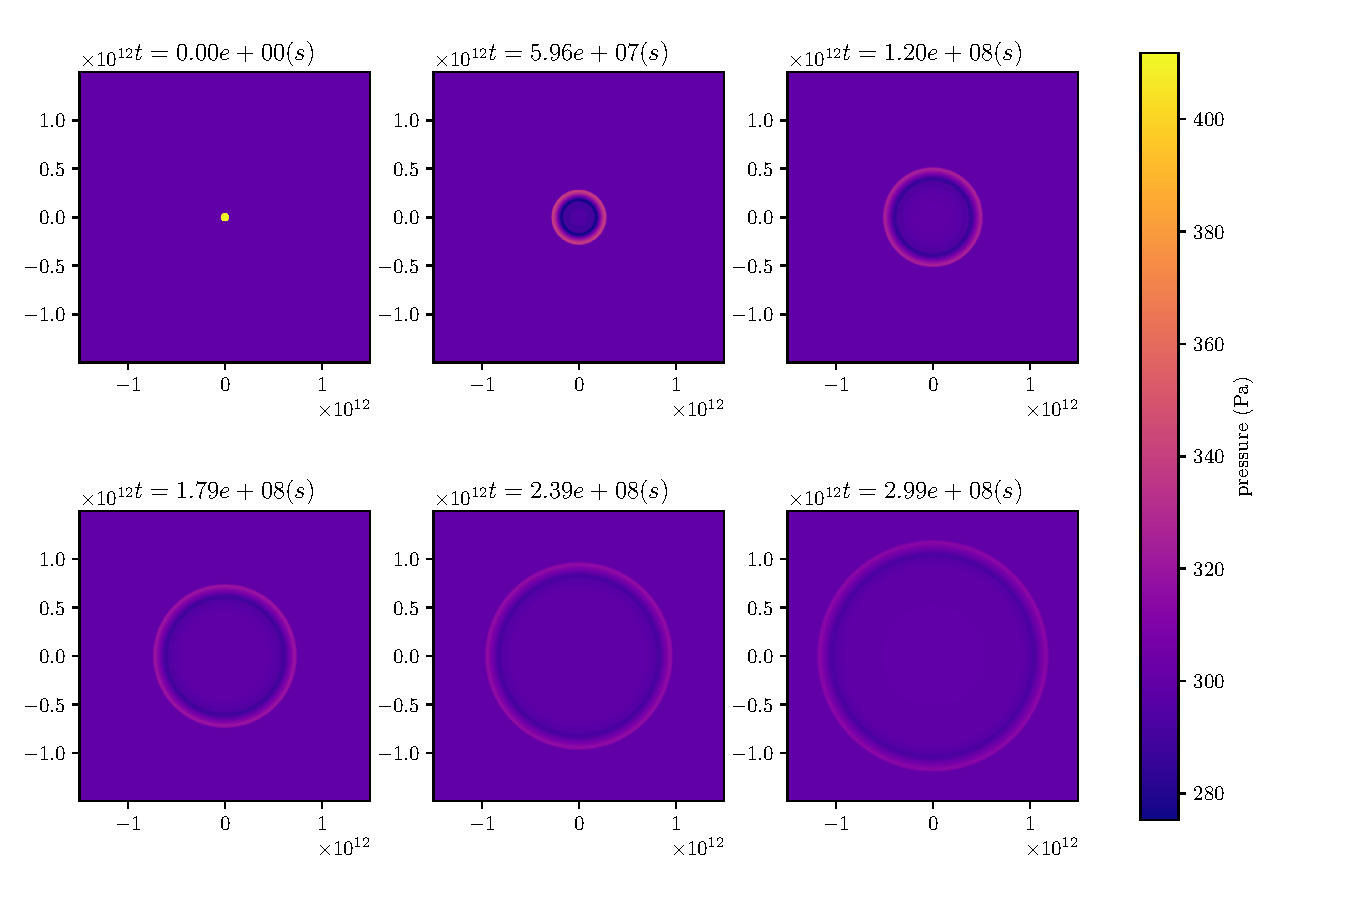
\includegraphics[width=\textwidth]{figures/blast_wave.pdf}
	\caption{Evolution of the pressure of the simulated blast wave. The $x$ and $y$-axis are in \si{cm}. Note that the colormap is cut off at $11$ code units and that the inital high pressure region is not faithfully represented.}
	\label{fig:blastwave}
\end{figure}

\Cref{fig:blastwave} shows pressure of the simulated fluid at multiple points in time. 
The speed at which the wave front moves is the group speed. 
According to \cref{sec:magnetohydrodynamics_and_the_solar_corona} this is given by $c_s = \sqrt{\frac{5}{3} \frac{p_0}{\rho_0}} $.
Hence the speed (in code units) is $\sqrt{\frac{5}{3}8} = 3.61$, which corresponds to \SI{3.61e5}{\centi\metre\per\second}.
A comparison of the theoretical radius against the simulated radius can be found in \cref{fig:wave_front_speed}. 
Note that the curve of the simulation is jagged because the grid on which the simulation is run is discreet. 
Initially the simulated wave moves faster than the theoretical group speed. 
This could be an result of the linear approximation used in determining the group speed.
However for the remainder of the simulation the wave front matches the theoretical group speed quite well.


\begin{figure}[h]
	\centering
	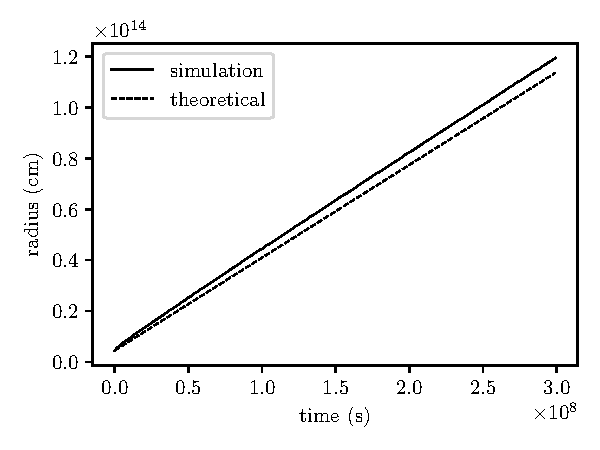
\includegraphics[width=0.5\textwidth]{figures/wavefront_position.pdf}
	\caption{The position of the simulated wave front compared to the theoretical speed}
	\label{fig:wave_front_speed}
\end{figure}

\subsection{Non-linear effects} \label{sec:nonlinear_effects}
Due to our current understanding of the (magnetic) navier-stokes equations, linear approximations are necessary for many theoretical results. 
This is one limitations of the theory that numerical simulations aim to solve.
A problem was setup with the same initial conditions as in \cref{sec:initial_example}, except that the initial pressure is 100 (code units) in the centre and 8 elsewhere. 
Like in the previous setup the radius of the blast over time was compared to the theoretically linear group speed.
\Cref{fig:non_linear_effects} shows concave radius/time relation against the linear theoretically predicted relation. 
\begin{figure}[h]
	\centering
	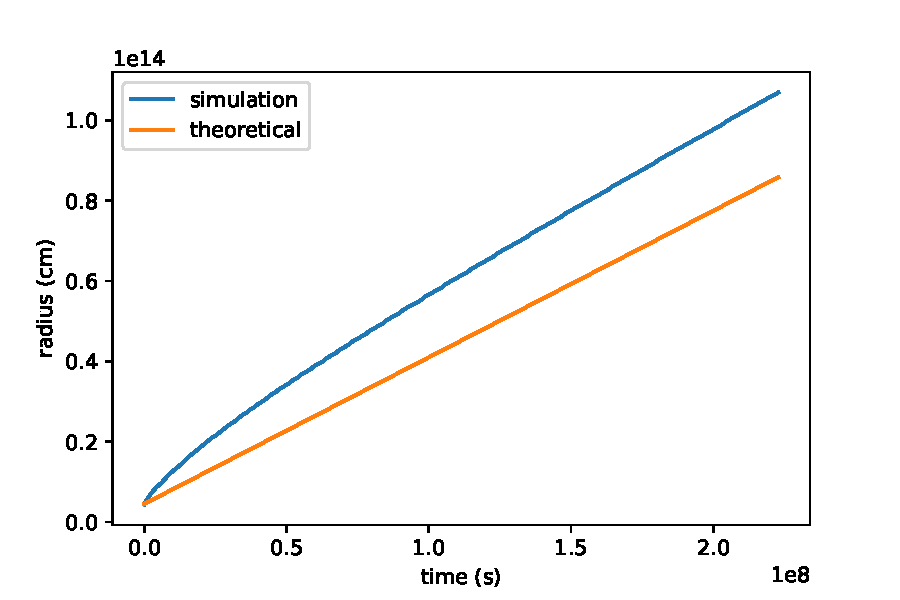
\includegraphics[width=0.5\textwidth]{figures/non_linear_effects.pdf}
	\caption{A comparison of the theoretically predicted radius of the blast wave (using a linear approximation) versus the simulated result}
	\label{fig:non_linear_effects}
\end{figure}

\pagebreak

\section{Waves in magnetohydrodynamic fluids} \label{sec:waves_in_magnetorhydrodynamic_fluids}
To simulate magnetohydrodynamic waves, PLUTO solves the following system of differential equations, which is slightly different from the one defined in \cref{sec:(m)hd_theory}.
\begin{alignat}{3}
    &\frac{\partial \rho}{\partial t} &&+ \nabla \cdot (\rho \mathbf v) &&= 0 \tag{mass}\label{masscontpluto}\\
    &\frac{\partial \mathbf m}{\partial t} &&+  \nabla \cdot \bigg[\mathbf{mv - BB+ I}\bigg(p + \frac{\mathbf B^2}{2}\bigg)\bigg]^T &&= -\rho \nabla \Phi + \rho\cdot g \tag{moment}\label{cauchymomentpluto}\\
    &\frac{\partial \mathbf B}{\partial t} &&+ \nabla \times (cE) &&= 0 \tag{charge}\label{Faradaypluto}\\
    &\frac{\partial(E_t + \rho \Phi)}{\partial t} &&+ \nabla \cdot \bigg[\bigg(\frac{\rho \mathbf v^2}{2} + \rho e + p + \rho \Phi\bigg)v + c \mathbf E \times \mathbf B\bigg] &&= m\cdot g \tag{energy}\label{energypluto}.
\end{alignat} 
Here $\rho$ is the plasma density, $\mathbf B$  the magnetic field,  $\mathbf v$ the velocity, $\mathbf m= \rho \mathbf v$ the momentum density, $\Phi$ the potential and $p$ is the thermal pressure. $E_t$ is the total energy, which is given by \[
E_t = \rho e + \frac{m^2}{2\rho} + \frac{B^2}{2}
.\]  
The constants  $e, c$ are the elementary charge and the speed of light respectively, and $\mathbf{E}$ is the electric field.\cite{plutouserguide}\\

In order to study the effects of a constant magnetic background field, the same initial conditions as in \cref{sec:initial_example} were used but this time a magnetic field in the $x$ direction was added. This can be done by adding a parameter $\beta$, and adjusting the \texttt{void init(...)} function in the \texttt{init.c} file as follows,
\begin{minted}
[frame=lines, bgcolor=mygray]
{c}
void Init (double *v, double x1, double x2, double x3){
  ...
  #if PHYSICS == MHD || PHYSICS == RMHD
  double g_beta = g_inputParam[BETA];
  v[BX1] = sqrt(g_inputParam[P_OUT]*2.0/g_beta);
  v[BX2] = 0.0;
  v[BX3] = 0.0;
  #endif
  ...
}
\end{minted}

The parameter $\beta = \frac{2p}{B^2}$ (in code units) gives the ratio of magnetic pressure over mechanical pressure. 
If $\beta = \infty$ the magnetic field is $0$. 
If $\beta \ll 1$ the magnetic pressure dominates. 

The simulation was run for 
\begin{itemize}
	\item 6 values for $\beta$ : $0.1, 0.3, 0.5, 1, 5, 10$
	\item 2 values for the high pressure region (in code units): $15, 100$ 
\end{itemize}
the background pressure was always $8$ code units.

\Cref{fig:blastwave_shape_beta} shows how the value of $\beta$ influences the shape of the blast wave. When $\beta$ is high, the blastwave resembles the ordinary non-magnetic hydrodynamics(\cref{fig:blastwave}).
\begin{figure}[H]
	\centering
	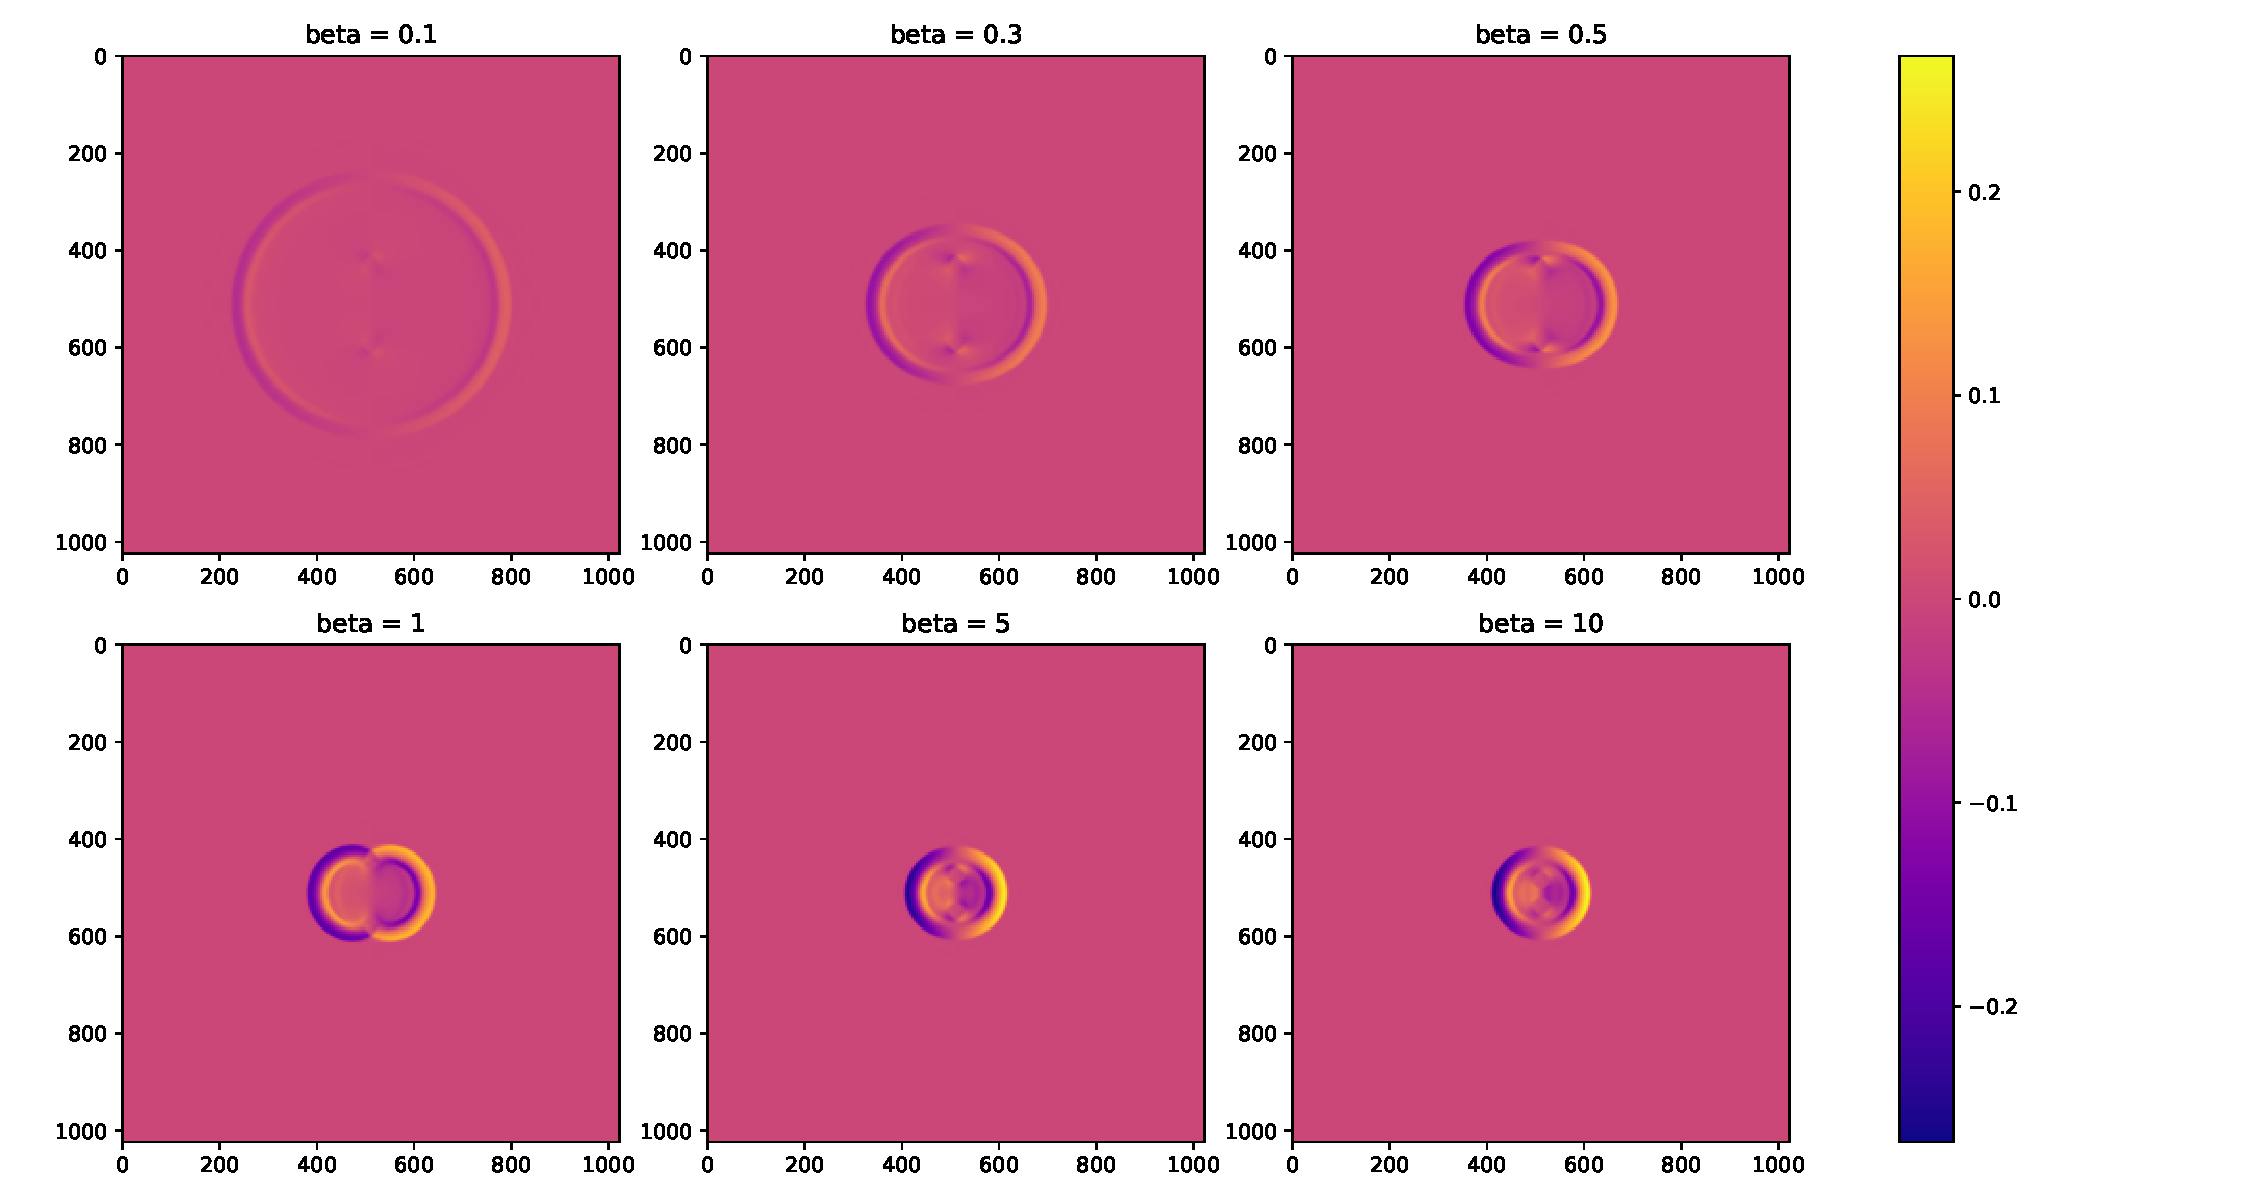
\includegraphics[width = \linewidth]{figures/influence_beta.pdf}
	\caption{The shape of the blast wave for different plasma beta's. Pressure is shown. The value for $\beta$ is modified with the thermal pressure held constant at $\SI{2995}{Ba}$ (8 code units) and constant density of 1 proton mass per  $\si{cm\cubed}$ (1 code unit). All figures are the simulation after $\SI{149597892}{s}$ (1 code units).}
\label{fig:blastwave_shape_beta}
\end{figure}

\Cref{fig:blastwave_shape_beta} very closely resembles the shape of the group speeds diagrams in \cref{fig:groupspeed_beta}. 
One can multiply the theoretical group speeds with the elapsed time to find the position of the high pressure region at that time. 
Overlaying \cref{fig:groupspeed_beta} with \cref{fig:blastwave_shape_beta} in this way results in \cref{fig:comparison_groupspeed}. One can see that they match very well. 
The experimental results are slightly ahead of the theoretical wavefront. The authors suspect that this is due two reasons:
\begin{enumerate}
	\item the theoretical position determines the movement of the centre of the initial high pressure region. But this has a non-zero radius. 
	\item the initial pressure difference (15 over 8 code units) is slightly to high for linear approximations. As a result the real group speed is higher than the linear theory would suggest.
\end{enumerate}

\begin{figure}[h]
	\centering
	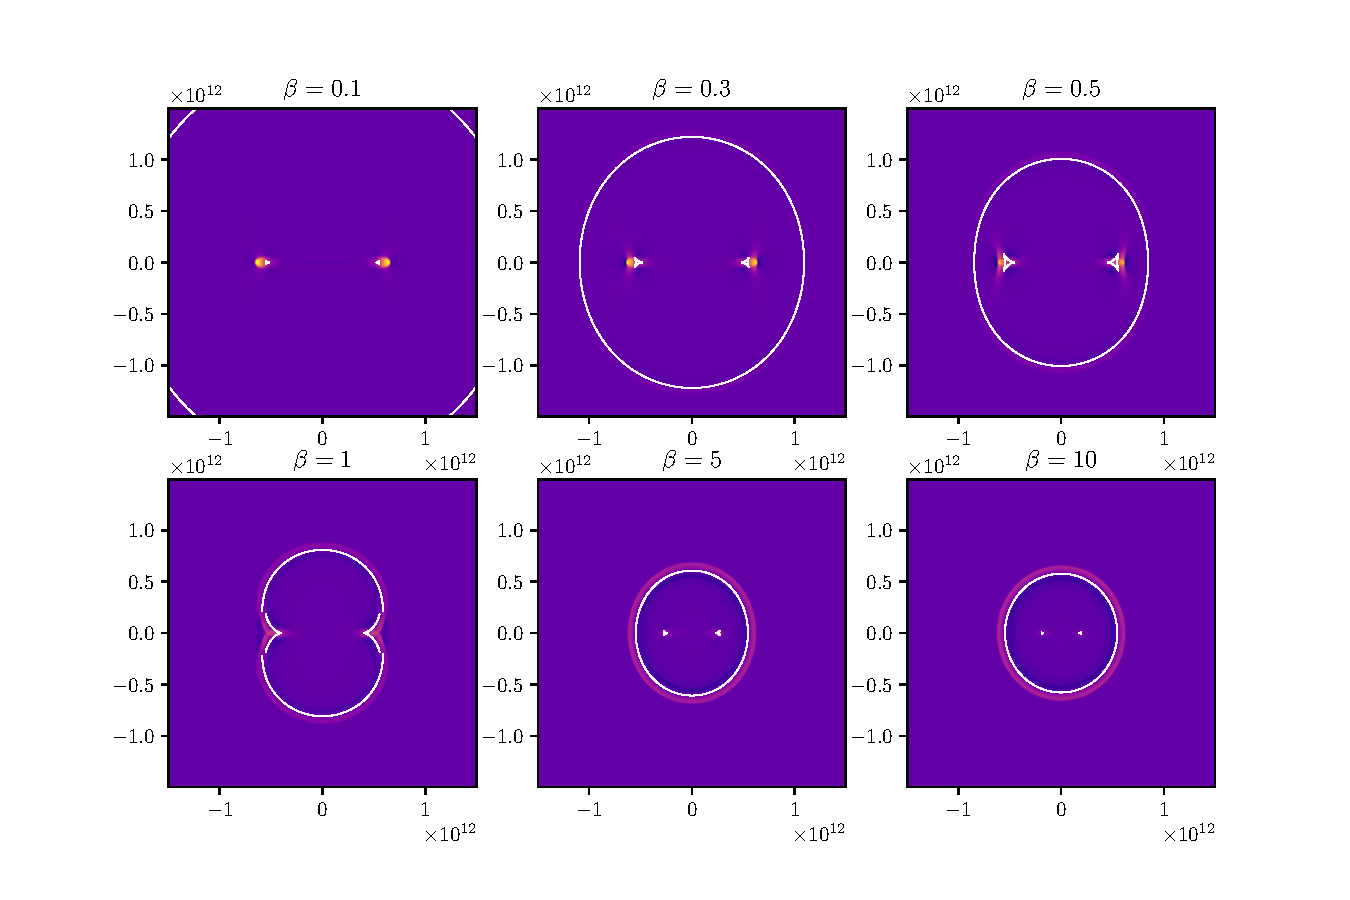
\includegraphics[width=\textwidth]{figures/comparison_groupspeed.pdf}
	\caption{The group speed diagrams (\cref{fig:groupspeed_beta}) overlayed on the simulations (\cref{fig:blastwave_shape_beta}). The white lines are the theoretical positions of the slow and fast magnetosonic wavefronts.}
	\label{fig:comparison_groupspeed}
\end{figure}
\todo{comparison sound speed theoretical vs simulation}


\subsection{Sound Waves}
\begin{figure}[H]
	\centering
	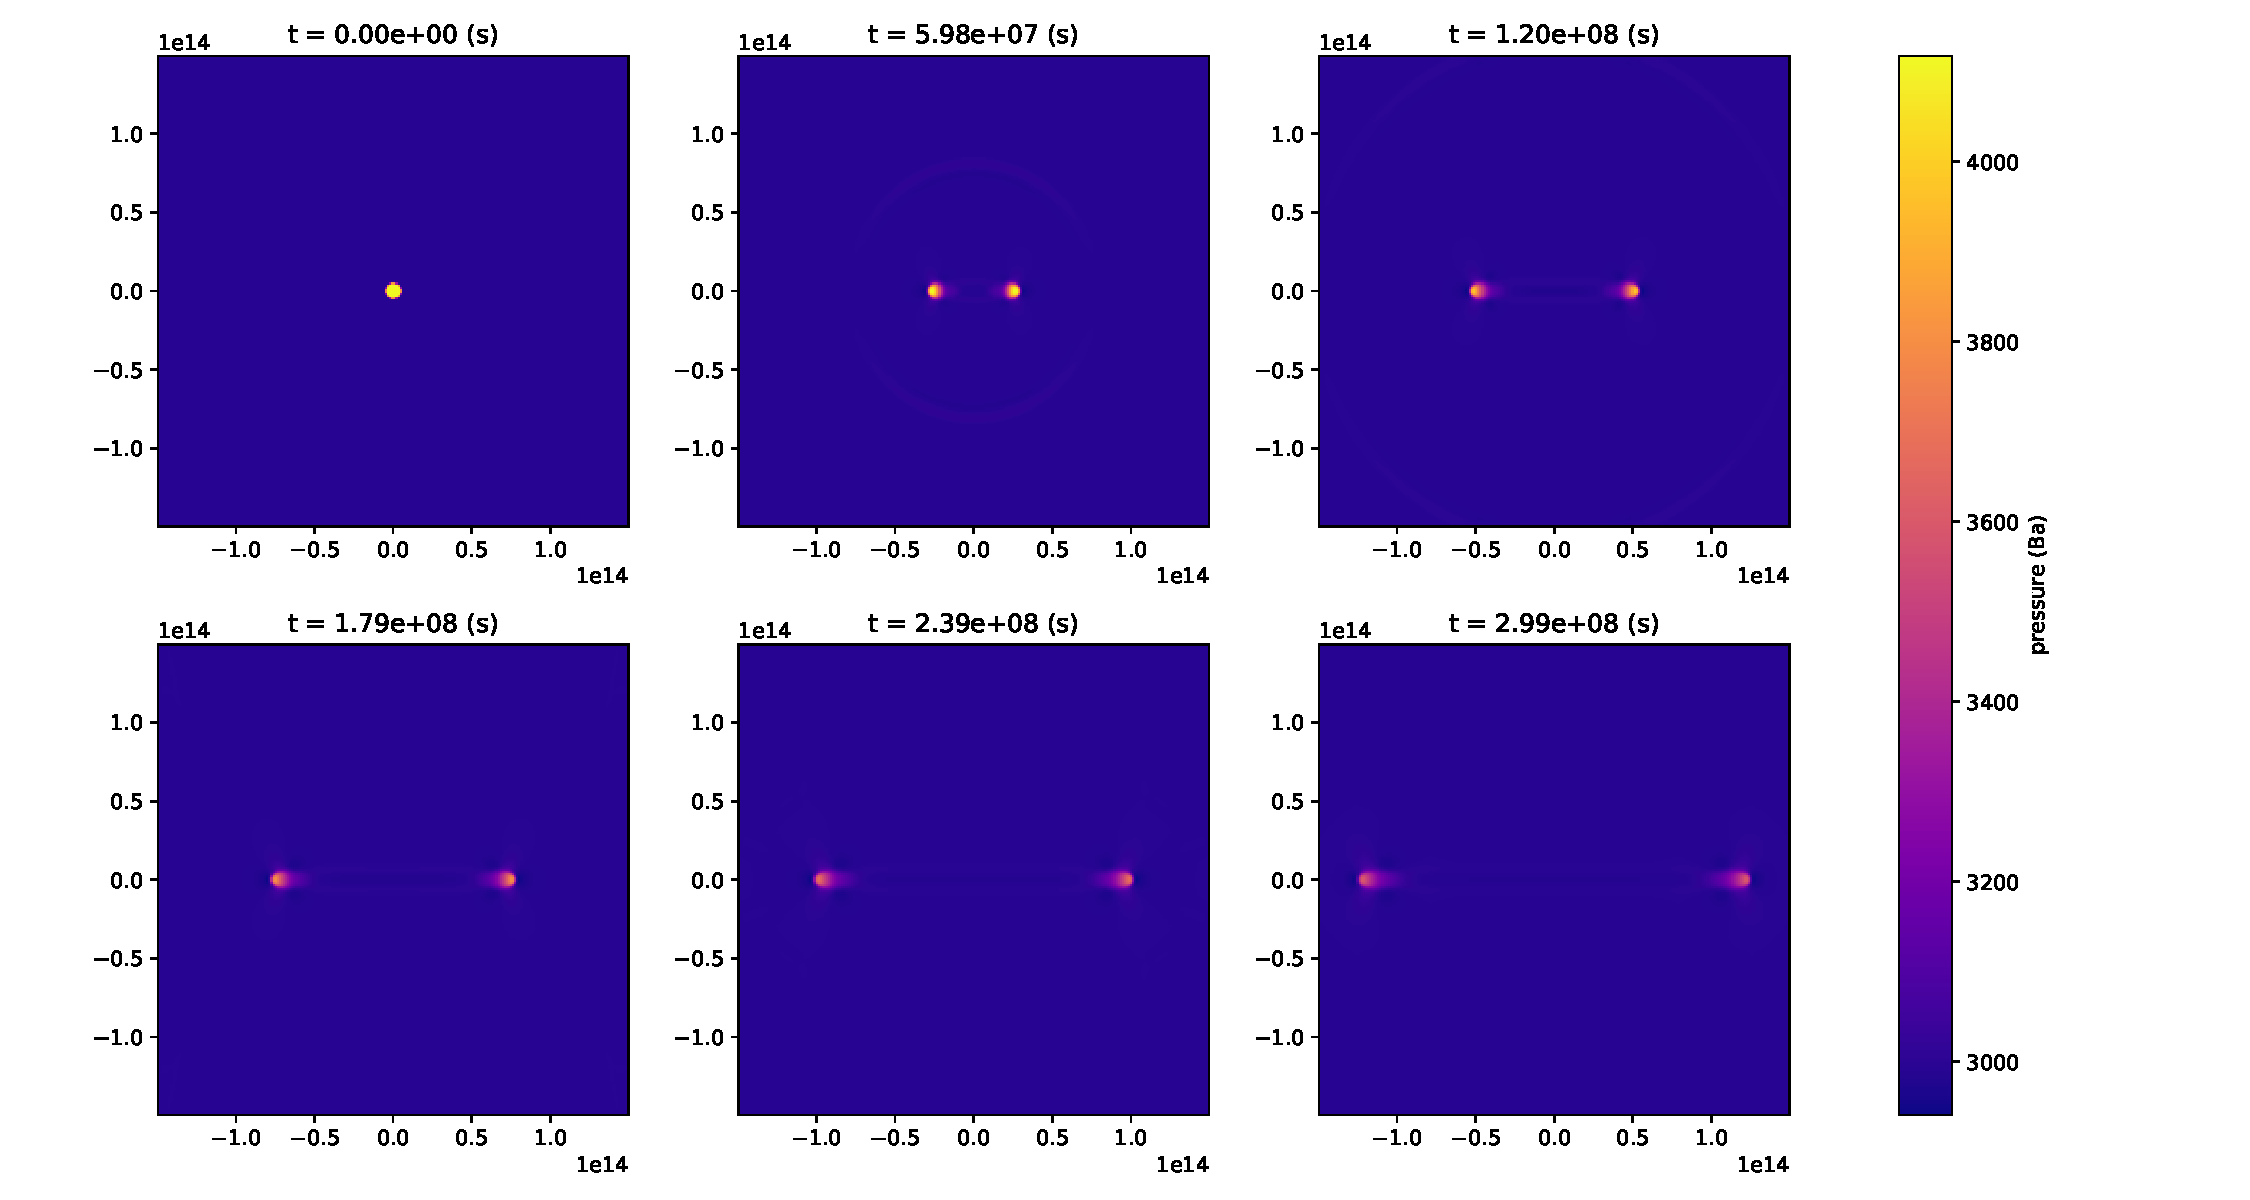
\includegraphics[width=\textwidth]{figures/slow_wave.pdf}
	\caption{The propagation of a slow wave. In this example $\beta = 0.1$ Axes are in \si{cm}.}
	\label{fig:Alfven_wave}
\end{figure}


In \cref{fig:Alfven_wave} the simulation results for the pressure of a magnetohydrodynamic blastwave with $\beta = 0.1$ are plotted, for different points in time. 
The simulation does not resemble that of a hydrodynamic blastwave, because $\beta$ is relatively small, which implies that the magnetic pressure dominates over the mechanical pressure.
In this simulation the fast magnetosonic wave is barely visible because it is faster and therefore a lot more dissipation takes place. \todo{ik heb mijn twijfels bij deze uitleg}
Hence this simulation can be used to compare the theoretical and 
experimental group speed of the slow wave.

Taking the right half of a horizontal slice and plotting over time is a good way of visualizing the propagation of the slow magnetosonic waves. This is visualised \cref{fig:slowwave_time} along with the theoretical boundary of the wave packet determined using the theoretical speed of the slow wave.  
Again the wave is slightly ahead of what theory predicts in the low pressure case. This is even more so for the high pressure blast. Again the authors think this discrepancy is due to non-linear effects.

\begin{figure}[h]
	\centering
	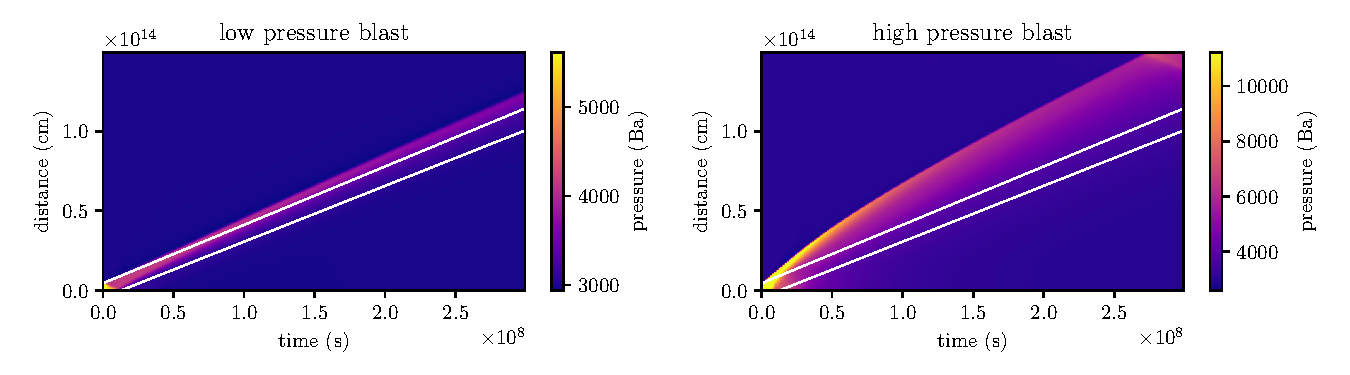
\includegraphics[width=1.1\textwidth]{figures/slowwave_time.pdf}
	\caption{The pressure of the a horizontal slice plotted over time of the HMD blastwave simulation with $\beta = 0.1$ for both the low and high pressure difference case. The white lines represent the theoretical bounds of the wave packet. The possible group speeds of a slow wave form a triangle as can be seen in \cref{fig:groupspeed_beta}. Taking let $v_m, v_M$ be the minimum and maximum speed in the $x$-direction of such a triangle. Let $r$ be the initial radius of the high pressure region. Then $x = v_m \cdot t - r, x = v_M \cdot t + r$ represent are the white boundaries.}
	\label{fig:slowwave_time}
\end{figure}
\pagebreak
\section{Interaction of MHD waves with large scale structures}
This task focuses on the interaction of large scale structures in the solar corona with magnetohydrodynamic waves and is based on the paper titled "Propagation of a global coronal wave and its interaction with large-scale coronal magnetic structures" by Afanasyev and Zhukov.  \cite{afanasyev2018propagation}\\

The shock wave simulated in \cref{sec:waves_in_magnetorhydrodynamic_fluids} is a good description of a wave in a uniform plasma, however it does not account for various large scale non-uniformities, such as coronal holes and plumes. The interaction of coronal waves with these structures results in wave phenomena such as wave transmission and reflection, which have been observed in extreme ultraviolet images of the Sun (see for example \cite{gopalswamy2009euv}).
\subsection{Coronal Hole Model}
A coronal hole, is a region of lower temperature and density compared to the surrounding plasma. This results in a region of higher Alfv\'en speed. They occur when a magnetic field does not fall back, and is open to interplanetary space \todo{Degelijke bron nodig}.\\

To simulate a coronal hole, the following initial conditions are used,
\begin{align*}
    n &= n_{\text{out}} - (n_{\text{out}}-n_{\text{in}})\exp\left[-\bigg(\frac{r}{d}\bigg)^8\right]\\
    T &= T_{\text{out}} - (T_{\text{out}}-T_{\text{in}})\exp\bigg[-\bigg(\frac{r}{d}\bigg)^8\bigg]
\end{align*}
Here $n$ denotes the plasma number density, $T$ denotes the temperature, and $r$ is the distance from the center. The parameter $d$ is used to describe the characteristic size of the non-uniformity and can hence be used to adjust the simulation to the correct order of magnitude. In this simulation $d$ will be equal to $150$ Mm (see also \cref{tab:coronal_hole}).\\

The magnetic field in the simulation is directed in the $z$-direction while the simulation takes place in the $x,y$-plane. An initial equilibrium is achieved by keeping the total pressure constant, using the following equation,
\begin{equation*}
    p^t = p_{\text{gas}} + \frac{B^2}{8\pi} = \text{constant}.
\end{equation*}
Here $p^t$ represents the total pressure, which is the sum of the gas pressure and the magnetic pressure. \\

A alven wave is induced by modifying the velocity in the $x$-direction in the boundary condition at the left boundary edge.
The velocity at the edge is given by \[
	v_x = v_\text{max}\tanh\left( \frac{t}{a_0} \right) - \frac{v_\text{max} }{2} \left(\tanh\left( \frac{t-d}{a_1} \right) + 1\right) 
,\]
where $t$ is the elapsed time,  $v_max$ the maximum speed obtained,  $d$ the duration of the wave. To avoid shocks, a hyperbolic tangent function is used to smoothly interpolate from 0 to $v_\text{max} $ and back. The values $a_0, a_1$ determine how fast it $v_x$ moves in between $0$ and $v_\text{max}$. 
In this report $a_0$ and $a_1$ will always be $\SI{20}{s}$ and $\SI{60}{s}$ respectively.
\Cref{fig:wave_drive} shows the velocity profile for these curves for both the coronal hole model and the coronal plume model (see \cref{sec:coronal_plume_model}).
\begin{figure}[h]
	\centering
	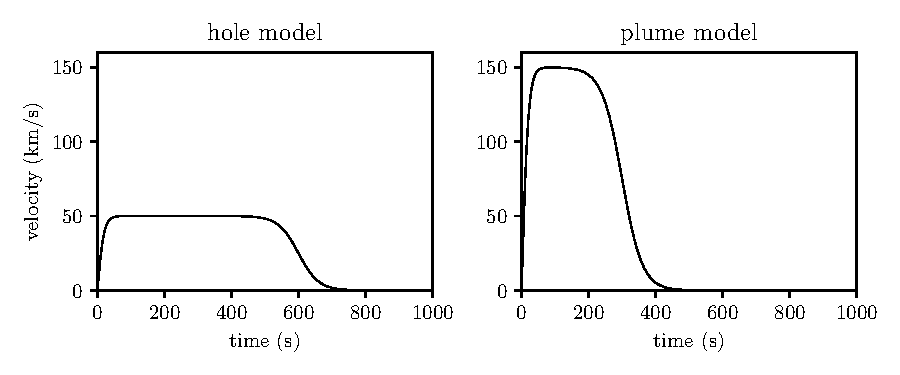
\includegraphics[width=0.8\textwidth]{figures/wave_drive}
	\caption{The velocity profile of the wave generated at the boundary of the coronal hole and coronal plume model.}
	\label{fig:wave_drive}
\end{figure}

The values that are used for the parameters are summarised in \cref{tab:coronal_hole}.
\begin{table}[H]
    \centering
    \caption{Parameters used to simulate the coronal hole model}
    \label{tab:coronal_hole}
    \begin{tabular}{|l|l|l|}
    \hline
    \textbf{Parameter}             & \textbf{Value}                                  & \textbf{Unit}              \\ \hline
    d                              & 150                                             & Mm                         \\ \hline
    $n_\text{out}$ & $1.0 \times 10^9$ & $\text{cm}^{-3}$ \\ \hline
    $n_\text{in}$                              & $1.0 \times 10^8$                                               & $\text{cm}^{-3}$                          \\ \hline
    $T_\text{out}$                              & 1.5                                               & \si{\mega\kelvin}                          \\ \hline
    $T_\text{in}$                              & 1.0                                               & \si{\mega\kelvin}                          \\ \hline
    $B_\text{out}$                              & 4.0                                               & G                          \\ \hline
    $v_\text{max}$ 			 	& 50						& \si{\kilo\metre \per \second}  \\ \hline
    $d$						& 600						& \si{\second} \\ \hline
\end{tabular}
\end{table}
To define these initial conditions the following adjustments have to be made to the \texttt{void init(...)} function in the \texttt{init.c} file. This code is an modified version of code kindly provided by Mijie Shi.
\begin{minted}
[frame=lines, breaklines, bgcolor=mygray]
{c}
void Init (double *v, double x1, double x2, double x3)
{ double rho_out, rho_ins, rho_all, T_out, T_ins, T_all, B_out, p_out, p_all;  //define some variables
  double d;
  double r;    

  d = g_inputParam[DIAM];
  rho_out = g_inputParam[RHO_OUT];
  rho_ins = g_inputParam[RHO_INS];
  T_out = g_inputParam[T_OUT];   //Physical value (Kelvin)
  T_ins = g_inputParam[T_INS];   //Physical value (Kelvin)
  
  r = sqrt(x1*x1 + x2*x2);    
  rho_all = rho_out - (rho_out - rho_ins)*exp(-(pow(r/d,8))); //density profile
  T_all = T_out - (T_out - T_ins)*exp(-(pow(r/d,8)));         //temperature profile

  p_out = rho_out*T_out/(KELVIN*0.5);                        //converitng from density and temperature to pressure 
  p_all = rho_all*T_all/(KELVIN*0.5);                        //KELVIN is defined by PLUTO 

  B_out = g_inputParam[B_OUT]/sqrt(4.0*CONST_PI*UNIT_DENSITY)/UNIT_VELOCITY;  //normalized magnetic field outside of the structure (physical value is 4 Gauss)
							      

  v[RHO] = rho_all;
  v[VX1] = 0.0;
  v[VX2] = 0.0;
  v[VX3] = 0.0;
  #if HAVE_ENERGY
  v[PRS] = p_all;
  #endif
  v[TRC] = 0.0;

  #if PHYSICS == MHD || PHYSICS == RMHD
  v[BX1] = 0.0;
  v[BX2] = 0.0;
  v[BX3] = sqrt(B_out*B_out + 2*(p_out - p_all));            //deriving the magnetic field from pressure balance, i.e., p + B^2/2 = const 

  v[AX1] = 0.0;
  v[AX2] = 0.0;
  v[AX3] = 0.0;
  #endif
}
\end{minted}
To generate a plane wave, the following time-dependent boundary condition is used at the right boundary of the simulation box. Firstly, two parameters are defined that make up the general shape of the wave namely, \texttt{WAVE\_HEIGHT}, which specifies the top speed of the wave, in km/s, and \texttt{WAVE\_DURATION}, which specifies the length of the wave. 

To initialise these boundary conditions in PLUTO, the following code is added to the \texttt{void UserDefBoundary(...)} function in the \texttt{init.c} file, again a modified version of the code by Mijie Shi.
\begin{minted}
[frame=lines,bgcolor=mygray,breaklines]
{c}
void UserDefBoundary (const Data *d, RBox *box, int side, Grid *grid){
  ...
  double v0, v1, v2, height, duration;
  height = g_inputParam[WAVE_HEIGHT];
  duration = g_inputParam[WAVE_DURATION];
  v0 = -height*1.e5/UNIT_VELOCITY;   
  v1 = -v0;
  v2 = 0.0;
  
  if (side == X1_BEG){  /* -- X1_BEG boundary -- */
    if (box->vpos == CENTER) {
      BOX_LOOP(box,k,j,i){ 
      d->Vc[RHO][k][j][i] = d->Vc[RHO][k][j][2*IBEG - i -1];
      d->Vc[PRS][k][j][i] = d->Vc[PRS][k][j][2*IBEG - i -1];
       
      d->Vc[BX1][k][j][i] = d->Vc[BX1][k][j][2*IBEG - i -1];
      d->Vc[BX2][k][j][i] = d->Vc[BX2][k][j][2*IBEG - i -1];
       
      d->Vc[VX1][k][j][i] = v1 + (v0 - v1)*(0.5*(1.-tanh((g_time-0.)/20.))) + (v2 - v1)*(0.5*(1.+tanh((g_time-duration)/60.)));
      
      d->Vc[VX2][k][j][i] = 0.0;
       
      }
    }else if (box->vpos == X1FACE){
      BOX_LOOP(box,k,j,i){  }
    }else if (box->vpos == X2FACE){
      BOX_LOOP(box,k,j,i){  }
    }else if (box->vpos == X3FACE){
      BOX_LOOP(box,k,j,i){  }
    }
  }
  ...
}
\end{minted}
The user defined parameters, the gridsize and resolution, output file type and timescale for the problem, can be defined in the \texttt{pluto.ini} file, similarly as in \cref{sec:initial_example}.
\begin{figure}[h]
	\centering
	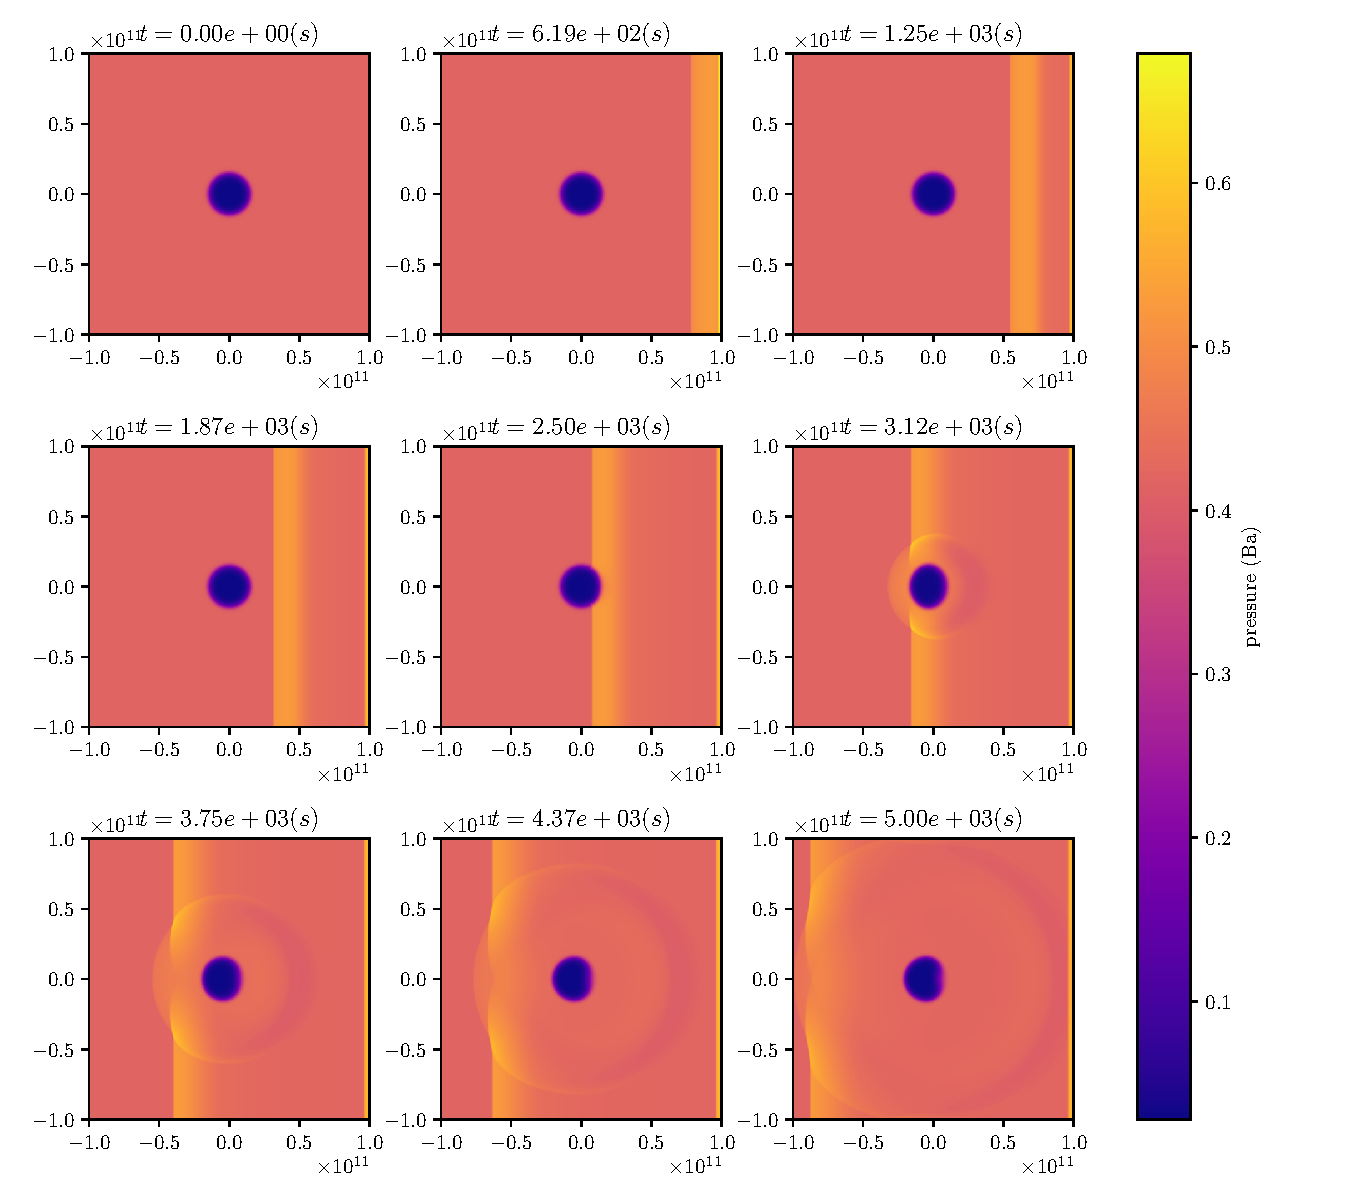
\includegraphics[width=1\textwidth]{figures/hole_time.pdf}
	\caption{}
	\label{fig:figures-hole}
\end{figure}
\subsection{Coronal Plume Model}\label{sec:coronal_plume_model} 
To contrast the coronal hole model, the plume model is considered. 
It is defined as a region of high temperature and density, and as a result a lower Alfv\'en speed.
This model is less applicable to real plumes, or collections of plumes, as the coronal hole model is to real coronal holes.\\

The simulation of the coronal plume consists of the same initial conditions as in the coronal hole simulation, namely,

\begin{align*}
    n &= n_{\text{out}} - (n_{\text{out}}-n_{\text{in}})\exp\left[-\bigg(\frac{r}{d}\bigg)^8\right]\\
    T &= T_{\text{out}} - (T_{\text{out}}-T_{\text{in}})\exp\bigg[-\bigg(\frac{r}{d}\bigg)^8\bigg]\\
     p^t &= p_{\text{gas}} + \frac{B^2}{8\pi} = \text{constant}.
\end{align*}
However, this time other values will be used for the parameters, alongside a smaller characteristic size ($d = 100$ Mm).
\begin{table}[H]
    \centering
    \caption{Parameters used to simulate the coronal plume model}
    \label{tab:coronal_plume}
    \begin{tabular}{|l|l|l|}
    \hline
    \textbf{Parameter}             & \textbf{Value}                                  & \textbf{Unit}              \\ \hline
    d                              & 100                                             & Mm                         \\ \hline
    $n_\text{out}$ & $1.0 \times 10^8$ & $\text{cm}^{-3}$ \\ \hline
    $n_\text{in}$                              & $1.0 \times 10^9$                                               & $\text{cm}^{-3}$                          \\ \hline
    $T_\text{out}$                              & 1.5                                               & MK                          \\ \hline
    $T_\text{in}$                              & 1.0                                               & MK                          \\ \hline
    $B_\text{out}$                              & 3.0                                               & G                          \\ \hline
    $v_\text{max}$ 			 	& 150						& \si{\kilo\metre \per \second}  \\ \hline
    $d$						& 300						& \si{\second} \\ \hline
\end{tabular}
\end{table}
To simulate the coronal plume, the same definition can be used, as the one for the coronal hole, by changing the parameters in the \texttt{definitions.h} file.\\

In \cref{fig:figures-plume_time-pdf} and \cref{fig:figures-plume_reflection-pdf} the simulation results for the interaction of a planar MHD wave with a coronal plume are plotted for different points in time. The pressure in the plots in  \cref{fig:figures-plume_time-pdf} is cut off at ???????? to increase the contrast of the waves outside of the plume. The opposite is done in \cref{fig:figures-plume_reflection-pdf}. \todo{Mss moet dit bij de beschrijving van de figuren?}.\\
\begin{figure}[h]
	\centering
	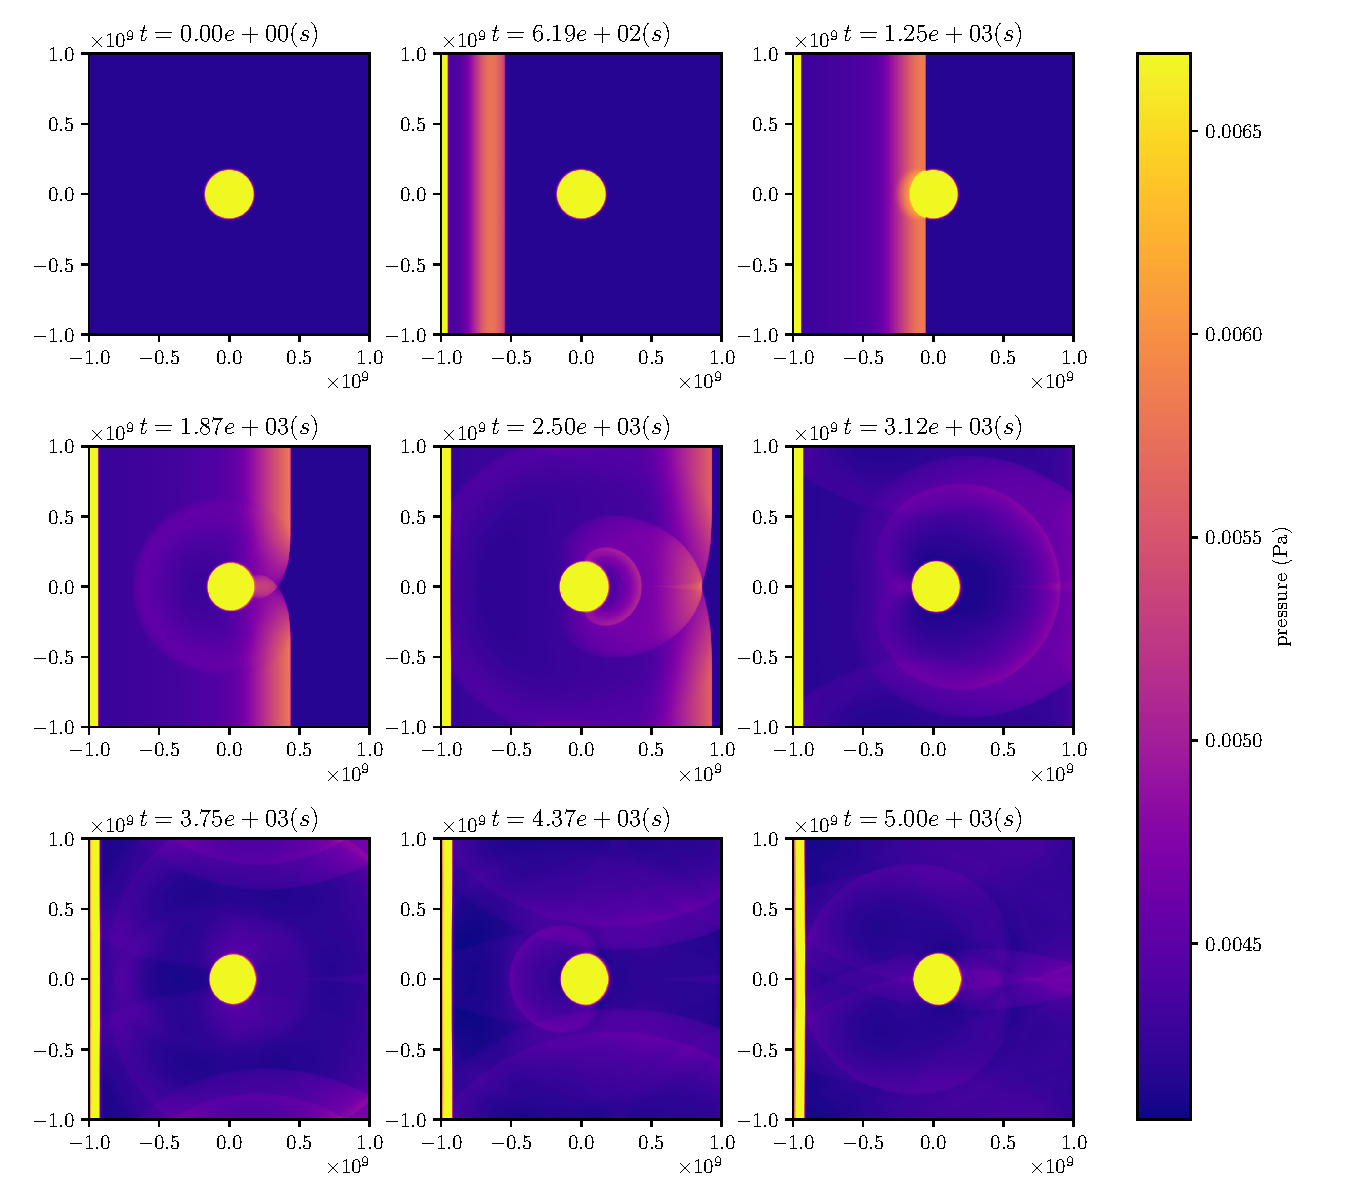
\includegraphics[width=1\textwidth]{figures/plume_time.pdf}
	\caption{}
	\label{fig:figures-plume_time-pdf}
\end{figure}
\begin{figure}[h]
    \centering
    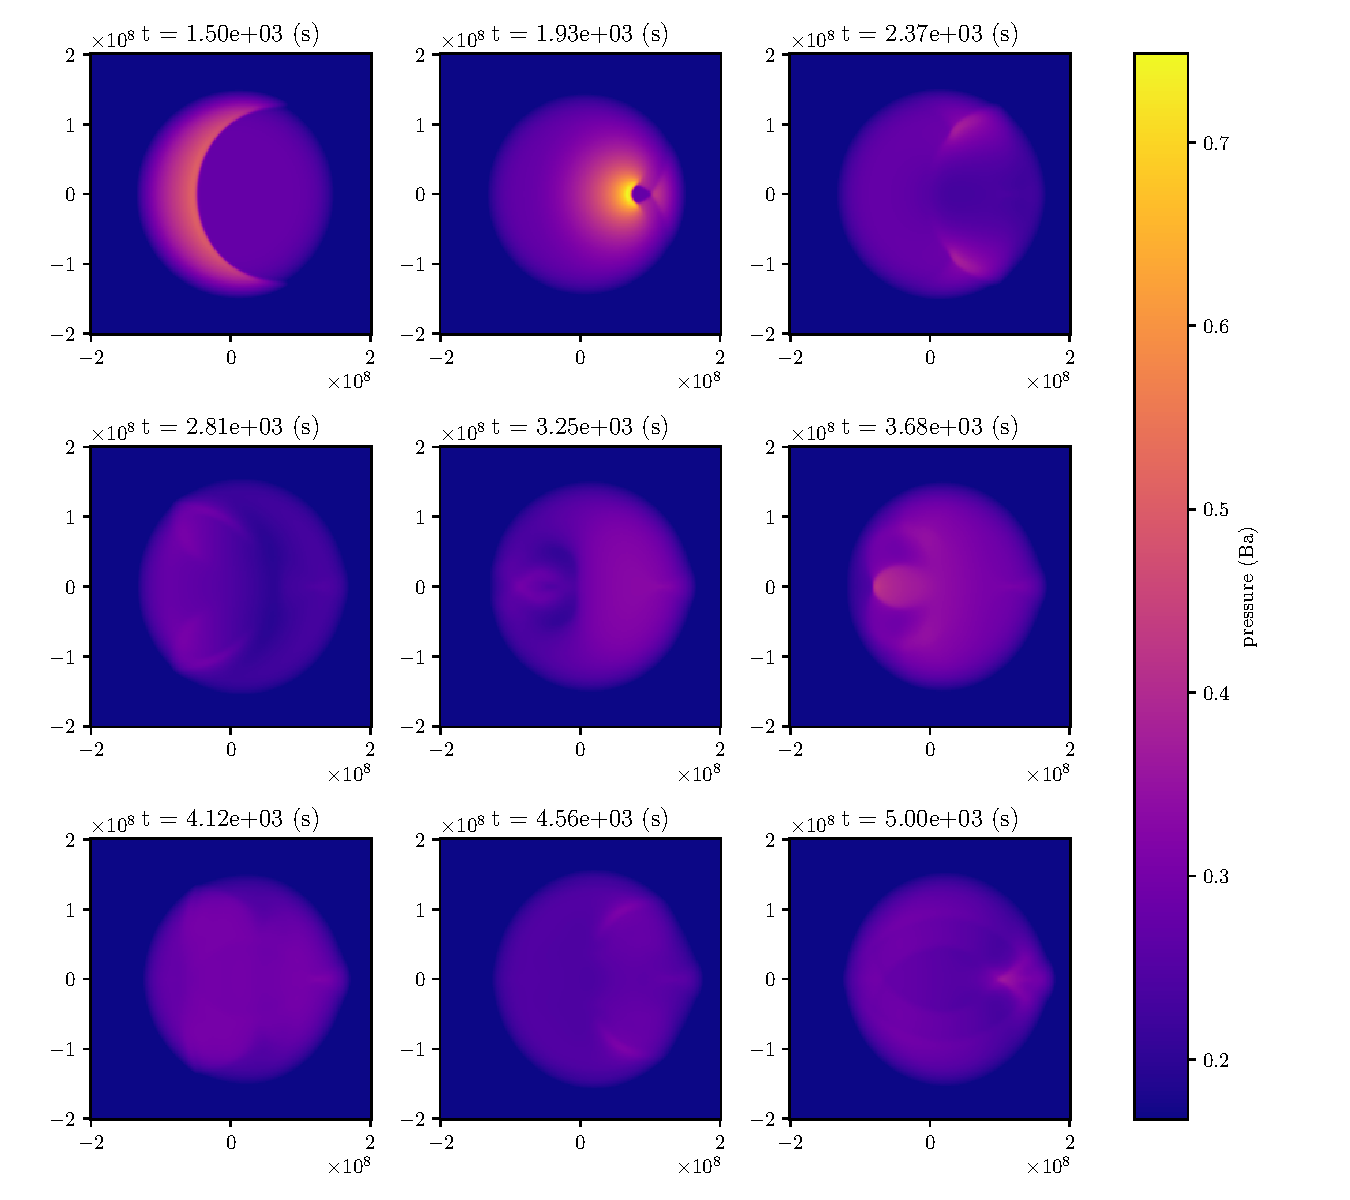
\includegraphics[width=1\textwidth]{figures/plume_reflection.pdf}
    \caption{}
    \label{fig:figures-plume_reflection-pdf}
\end{figure}
When the wave front passes through the plume, it is reflected because of the large difference in density of the plume and its surroundings. This reflection is in turn reflected again on the other side of the plume, causing a resonating effect visible in \cref{fig:figures-plume_reflection-pdf}. This ``captured'' wave, generates secondary wave fronts, visible in \cref{fig:figures-plume_time-pdf}.
\printbibliography
\end{document}
